\documentclass[12pt,a4paper]{report}

% ============================================================
%  PACKAGES
% ============================================================
\usepackage[utf8]{inputenc}
\usepackage[T1]{fontenc}
\usepackage{lmodern}
\usepackage[margin=2.5cm, top=3cm, bottom=3cm]{geometry}
\usepackage{graphicx}
\usepackage{xcolor}
\usepackage{tikz}
\usetikzlibrary{shapes, arrows.meta, positioning, calc, fit, backgrounds, decorations.pathreplacing}
\usepackage{tcolorbox}
\tcbuselibrary{skins, breakable, listings}
\usepackage{listings}
\usepackage{booktabs}
\usepackage{array}
\usepackage{tabularx}
\usepackage{multirow}
\usepackage{colortbl}
\usepackage{enumitem}
\usepackage{fancyhdr}
\usepackage{titlesec}
\usepackage{hyperref}
\usepackage{amsmath, amssymb}
\usepackage{float}
\usepackage{caption}
\usepackage{setspace}
\usepackage{parskip}

% ============================================================
%  COLOR DEFINITIONS (matching Database SQL style)
% ============================================================
\definecolor{chapterblue}{RGB}{0, 82, 155}
\definecolor{sectionblue}{RGB}{0, 82, 155}
\definecolor{defblue}{RGB}{0, 102, 179}
\definecolor{defbg}{RGB}{222, 239, 252}
\definecolor{defborder}{RGB}{150, 200, 235}
\definecolor{infobg}{RGB}{222, 239, 252}
\definecolor{infoborder}{RGB}{100, 160, 220}
\definecolor{warningbg}{RGB}{255, 243, 224}
\definecolor{warningborder}{RGB}{230, 160, 60}
\definecolor{warningheader}{RGB}{220, 120, 20}
\definecolor{importantbg}{RGB}{230, 248, 230}
\definecolor{importantborder}{RGB}{80, 180, 80}
\definecolor{conceptbg}{RGB}{240, 237, 252}
\definecolor{conceptborder}{RGB}{120, 100, 190}
\definecolor{codebg}{RGB}{248, 248, 248}
\definecolor{codeborder}{RGB}{80, 80, 80}
\definecolor{cppkeyword}{RGB}{0, 0, 200}
\definecolor{cppcomment}{RGB}{0, 128, 0}
\definecolor{cppstring}{RGB}{200, 0, 0}
\definecolor{cpppreproc}{RGB}{128, 0, 128}
\definecolor{borderblue}{RGB}{0, 102, 179}
\definecolor{headergray}{RGB}{100, 100, 100}
\definecolor{tableheader}{RGB}{0, 102, 179}
\definecolor{tableheadtext}{RGB}{255, 255, 255}
\definecolor{coverred}{RGB}{180, 30, 30}
\definecolor{lightgray}{RGB}{245, 245, 245}

% ============================================================
%  PAGE STYLE & HEADERS
% ============================================================
\pagestyle{fancy}
\fancyhf{}
\fancyhead[L]{\small\textsc{\nouppercase{\leftmark}}}
\fancyhead[R]{\small\textcolor{headergray}{Al-Mustafa University $|$ Dept.\ of AI}}
\fancyfoot[C]{%
    \begin{tikzpicture}[baseline={(current bounding box.north)}]
        \draw[borderblue, line width=0.4pt] (0,0) -- (\textwidth,0);
        \node[anchor=north] at (0.5\textwidth, -2pt) {\small\thepage};
    \end{tikzpicture}%
}
\renewcommand{\headrulewidth}{0pt}% we draw our own
\renewcommand{\footrulewidth}{0pt}% we draw our own via tikz

% Custom blue header rule
\makeatletter
\renewcommand{\headrule}{%
    \vspace{-4pt}%
    {\color{borderblue}\hrule width\headwidth height 1.2pt}%
}
\makeatother

\fancypagestyle{plain}{
    \fancyhf{}
    \fancyfoot[C]{%
        \begin{tikzpicture}[baseline={(current bounding box.north)}]
            \draw[borderblue, line width=0.4pt] (0,0) -- (\textwidth,0);
            \node[anchor=north] at (0.5\textwidth, -2pt) {\small\thepage};
        \end{tikzpicture}%
    }
    \renewcommand{\headrulewidth}{0pt}
    \renewcommand{\footrulewidth}{0pt}
}

% ============================================================
%  CHAPTER & SECTION FORMATTING
% ============================================================
\titleformat{\chapter}[display]
    {\normalfont\bfseries\centering}
    {%
        \tikz[baseline]{%
            \node[inner sep=6pt, text=chapterblue] {\small\textsc{CHAPTER \thechapter}};%
            \draw[borderblue, line width=0.6pt] (-2,-.15) -- (2,-.15);%
        }%
    }
    {6pt}
    {\Huge\color{chapterblue}}
\titlespacing*{\chapter}{0pt}{-10pt}{35pt}

\titleformat{\section}
    {\normalfont\Large\bfseries\color{sectionblue}}
    {\thesection}{1em}{}

\titleformat{\subsection}
    {\normalfont\large\bfseries\color{sectionblue!80!black}}
    {\thesubsection}{1em}{}

\titleformat{\subsubsection}
    {\normalfont\normalsize\bfseries}
    {\thesubsubsection}{1em}{}

% ============================================================
%  TABLE STYLING - Blue header rows with white text
% ============================================================
\newcommand{\tableheaderrow}{\rowcolor{tableheader}}
\newcommand{\tablehead}[1]{\textcolor{tableheadtext}{\textbf{#1}}}

% ============================================================
%  CUSTOM TCOLORBOX ENVIRONMENTS
% ============================================================

% --- Definition Box (light blue, like Database SQL style) ---
\newtcolorbox{definitionbox}[1]{
    enhanced,
    breakable,
    colback=defbg,
    colframe=defborder,
    coltitle=white,
    fonttitle=\bfseries\small,
    title={\colorbox{defblue}{\strut\hspace{3pt}Definition: #1\hspace{3pt}}},
    attach boxed title to top left={yshift=-2mm, xshift=2mm},
    boxed title style={
        colback=defblue,
        sharp corners,
        boxrule=0pt,
    },
    top=8mm,
    left=4mm,
    right=4mm,
    bottom=4mm,
    boxrule=0.5pt,
    arc=1mm,
}

% --- Info Box (blue) ---
\newtcolorbox{infobox}[1]{
    enhanced,
    breakable,
    colback=infobg,
    colframe=infoborder,
    coltitle=white,
    fonttitle=\bfseries\small,
    title={\colorbox{infoborder}{\strut\hspace{3pt}#1\hspace{3pt}}},
    attach boxed title to top left={yshift=-2mm, xshift=2mm},
    boxed title style={
        colback=infoborder,
        sharp corners,
        boxrule=0pt,
    },
    top=8mm,
    left=4mm,
    right=4mm,
    bottom=4mm,
    boxrule=0.5pt,
    arc=1mm,
}

% --- Warning Box (orange) ---
\newtcolorbox{warningbox}[1]{
    enhanced,
    breakable,
    colback=warningbg,
    colframe=warningborder,
    coltitle=white,
    fonttitle=\bfseries\small,
    title={\colorbox{warningheader}{\strut\hspace{3pt}#1\hspace{3pt}}},
    attach boxed title to top left={yshift=-2mm, xshift=2mm},
    boxed title style={
        colback=warningheader,
        sharp corners,
        boxrule=0pt,
    },
    top=8mm,
    left=4mm,
    right=4mm,
    bottom=4mm,
    boxrule=0.5pt,
    arc=1mm,
}

% --- Important Box (green) ---
\newtcolorbox{importantbox}[1]{
    enhanced,
    breakable,
    colback=importantbg,
    colframe=importantborder,
    coltitle=white,
    fonttitle=\bfseries\small,
    title={\colorbox{importantborder}{\strut\hspace{3pt}#1\hspace{3pt}}},
    attach boxed title to top left={yshift=-2mm, xshift=2mm},
    boxed title style={
        colback=importantborder,
        sharp corners,
        boxrule=0pt,
    },
    top=8mm,
    left=4mm,
    right=4mm,
    bottom=4mm,
    boxrule=0.5pt,
    arc=1mm,
}

% --- Concept Box (purple/lavender) ---
\newtcolorbox{conceptbox}[1]{
    enhanced,
    breakable,
    colback=conceptbg,
    colframe=conceptborder,
    coltitle=white,
    fonttitle=\bfseries\small,
    title={\colorbox{conceptborder}{\strut\hspace{3pt}#1\hspace{3pt}}},
    attach boxed title to top left={yshift=-2mm, xshift=2mm},
    boxed title style={
        colback=conceptborder,
        sharp corners,
        boxrule=0pt,
    },
    top=8mm,
    left=4mm,
    right=4mm,
    bottom=4mm,
    boxrule=0.5pt,
    arc=1mm,
}

% ============================================================
%  C++ CODE LISTING STYLE
% ============================================================
\lstdefinestyle{cppstyle}{
    language=C++,
    basicstyle=\ttfamily\small,
    keywordstyle=\color{cppkeyword}\bfseries,
    commentstyle=\color{cppcomment}\itshape,
    stringstyle=\color{cppstring},
    directivestyle=\color{cpppreproc},
    showstringspaces=false,
    breaklines=true,
    breakatwhitespace=true,
    tabsize=4,
    frame=none,
    numbers=none,
    xleftmargin=4mm,
    xrightmargin=2mm,
    aboveskip=2mm,
    belowskip=2mm,
    morekeywords={cout, cin, endl, string, include, iostream, cmath, cstring, cstdlib, ctype, void, int, float, double, char, long, return, if, else, for, while, do, switch, case, break, default, struct, typedef, const, true, false, NULL, sizeof, bool, auto, class, namespace, using, std, new, delete, try, catch, throw, template, typename, virtual, override, public, private, protected},
}

\newtcblisting{cppcode}{
    enhanced,
    breakable,
    colback=codebg,
    colframe=codeborder,
    boxrule=0pt,
    leftrule=3pt,
    arc=0mm,
    left=2mm,
    right=2mm,
    top=2mm,
    bottom=2mm,
    listing only,
    listing options={style=cppstyle},
}

% Inline code style
\newcommand{\code}[1]{\texttt{\small\color{cppkeyword}#1}}

% ============================================================
%  WATERMARK (diagonal text like the original)
% ============================================================
% Uncomment below to add watermark
% \usepackage{draftwatermark}
% \SetWatermarkText{Dr.~Husam Salah Mahdi}
% \SetWatermarkScale{0.4}
% \SetWatermarkAngle{45}
% \SetWatermarkColor[gray]{0.9}

% ============================================================
%  HYPERREF SETUP
% ============================================================
\hypersetup{
    colorlinks=true,
    linkcolor=chapterblue,
    urlcolor=chapterblue,
    citecolor=chapterblue,
    pdftitle={Structured Programming C++ - Enhanced Edition},
    pdfauthor={Dr. Husam Salah Mahdi},
}

% ============================================================
%  DOCUMENT START
% ============================================================
\begin{document}

% ============================================================
%  COVER PAGE
% ============================================================
\begin{titlepage}
\begin{tikzpicture}[remember picture, overlay]
    % --- Outer thick border ---
    \draw[line width=3pt, borderblue]
        ([xshift=10mm, yshift=-10mm]current page.north west)
        rectangle
        ([xshift=-10mm, yshift=10mm]current page.south east);
    % --- Inner thin border ---
    \draw[line width=0.5pt, borderblue]
        ([xshift=13mm, yshift=-13mm]current page.north west)
        rectangle
        ([xshift=-13mm, yshift=13mm]current page.south east);

    % ======== FOUR CORNER TRIANGULAR DECORATIONS ========

    % --- Top-Left decorative triangle ---
    \fill[borderblue]
        ([xshift=10mm, yshift=-10mm]current page.north west)
        -- ++(0, -28mm)
        -- ++(14mm, 28mm)
        -- cycle;

    % --- Top-Right decorative triangle ---
    \fill[borderblue]
        ([xshift=-10mm, yshift=-10mm]current page.north east)
        -- ++(0, -28mm)
        -- ++(-14mm, 28mm)
        -- cycle;

    % --- Bottom-Left decorative triangle ---
    \fill[borderblue]
        ([xshift=10mm, yshift=10mm]current page.south west)
        -- ++(0, 28mm)
        -- ++(14mm, -28mm)
        -- cycle;

    % --- Bottom-Right decorative triangle ---
    \fill[borderblue]
        ([xshift=-10mm, yshift=10mm]current page.south east)
        -- ++(0, 28mm)
        -- ++(-14mm, -28mm)
        -- cycle;
\end{tikzpicture}

\centering
\vspace*{1.2cm}

% University Logo

\includegraphics[width=3.5cm]{logo.png}

\vspace{0.6cm}

{\Large\bfseries Al-Mustafa University}\\[4pt]
{\normalsize Department of AI}

\vspace{0.8cm}

% Red decorative rule above title
{\color{coverred}\rule{0.75\textwidth}{2pt}}

\vspace{0.7cm}

{\fontsize{34}{40}\selectfont\bfseries\color{chapterblue} Structured Programming}\\[10pt]
{\fontsize{34}{40}\selectfont\bfseries\color{chapterblue} C++}

\vspace{0.6cm}

% Red decorative rule below title
{\color{coverred}\rule{0.75\textwidth}{2pt}}

\vspace{0.7cm}

{\Large\bfseries\color{chapterblue} Part I: Theory Section}

\vspace{0.5cm}

{\normalsize ECTS Credits: 8}\\[3pt]
{\normalsize Module Level: 1 $|$ Semester: 2}

\vspace{1.2cm}

% Instructor block with subtle blue accent

\begin{tikzpicture}
    \node[inner sep=8pt] (instructor) {%
        \begin{minipage}{0.5\textwidth}
            \centering
            {\large\bfseries Instructor}\\[5pt]
            {\large Dr.\ Husam Salah Mahdi}\\[3pt]
            {\normalsize HOD AI Dep}
        \end{minipage}
    };
    \draw[borderblue, line width=0.5pt] (instructor.north west) -- (instructor.north east);
    \draw[borderblue, line width=0.5pt] (instructor.south west) -- (instructor.south east);
\end{tikzpicture}

\vspace{0.8cm}

{\normalsize First Year -- Second Course}\\[3pt]
{\normalsize Academic Year: 2025--2026}

\vspace*{\fill}
\end{titlepage}

% ============================================================
%  PART I PAGE
% ============================================================
\newpage
\thispagestyle{empty}
\begin{tikzpicture}[remember picture, overlay]
    % Subtle blue gradient band at top
    \fill[borderblue!15] (current page.north west) rectangle ([yshift=-3cm]current page.north east);
    \draw[borderblue, line width=1.5pt] ([yshift=-3cm]current page.north west) -- ([yshift=-3cm]current page.north east);
    % Subtle blue band at bottom
    \fill[borderblue!15] (current page.south west) rectangle ([yshift=2cm]current page.south east);
    \draw[borderblue, line width=1.5pt] ([yshift=2cm]current page.south west) -- ([yshift=2cm]current page.south east);
\end{tikzpicture}

\vspace*{\fill}
\begin{center}
    {\color{borderblue}\rule{0.4\textwidth}{1pt}}\\[15pt]
    {\fontsize{42}{50}\selectfont\bfseries\color{chapterblue} Part I}\\[20pt]
    {\LARGE\bfseries\color{chapterblue} Theory Section}\\[15pt]
    {\color{borderblue}\rule{0.4\textwidth}{1pt}}
\end{center}
\vspace*{\fill}
\newpage

% ============================================================
%  TABLE OF CONTENTS
% ============================================================
\tableofcontents
\newpage

% ============================================================
%  CHAPTERS
% ============================================================

%=============================================================================
% Chapter 1: Functions in C++
% Structured Programming with C++ -- Lectures 11-12
%=============================================================================

\chapter{Functions in C++}
\label{ch:functions}

%-----------------------------------------------------------------------------
\section{Introduction to Functions}
\label{sec:intro-functions}
%-----------------------------------------------------------------------------

\begin{definitionbox}{Function}
A \textbf{function} is a self-contained set of statements designed to accomplish
a particular task. Every C++ program contains at least one function ---
\texttt{main()} --- and may define any number of additional functions.
\end{definitionbox}

In practice, large programs are difficult to write, read, and maintain as a
single monolithic block of code. The solution is \emph{modular programming}:
dividing a program into smaller, manageable pieces called \textbf{functions}.
Each function performs a specific, well-defined task, and the complete program
is built by combining these functions together.

\begin{infobox}{Advantages of Using Functions}
\begin{enumerate}
    \item \textbf{Easier to write:} Each function focuses on a single task,
          making the logic simpler to implement.
    \item \textbf{Easier to read:} Well-named functions make the overall
          program flow self-documenting and understandable at a glance.
    \item \textbf{Easier to debug:} Errors can be isolated to individual
          functions, reducing the search space during troubleshooting.
    \item \textbf{Reusability:} A function can be called multiple times with
          different parameters, eliminating code duplication.
    \item \textbf{Team development:} Different programmers can work on
          different functions simultaneously.
\end{enumerate}
\end{infobox}

\begin{conceptbox}{Modular Programming}
Modular programming is a software design technique that decomposes a program
into separate sub-programs (modules or functions). Each module is developed
and tested independently, then integrated into the complete program. This
approach reduces complexity and improves code quality.
\end{conceptbox}

%-----------------------------------------------------------------------------
\section{Defining a Function}
\label{sec:defining-function}
%-----------------------------------------------------------------------------

Every function definition in C++ consists of four parts: a \textbf{return type},
a \textbf{function name}, a \textbf{parameter list}, and a \textbf{function
body}. The general form is:

\begin{cppcode}
return-type function-name(parameter-list)
{
    // body of the function
    statement1;
    statement2;
    ...
    return value;  // (if return-type is not void)
}
\end{cppcode}

\begin{importantbox}{Components of a Function Definition}
\begin{itemize}
    \item \textbf{Return type:} The data type of the value returned by the
          function. Common types include \texttt{int}, \texttt{float},
          \texttt{double}, \texttt{char}, and \texttt{void} (when the function
          returns nothing).
    \item \textbf{Function name:} A valid C++ identifier that describes the
          purpose of the function.
    \item \textbf{Parameter list:} A comma-separated list of typed variables
          that receive values from the caller. May be empty if the function
          requires no input.
    \item \textbf{Function body:} The block of statements enclosed in braces
          \texttt{\{\}} that define what the function does.
\end{itemize}
\end{importantbox}

%-----------------------------------------------------------------------------
\subsection{Function Prototype (Declaration)}
\label{subsec:function-prototype}
%-----------------------------------------------------------------------------

A \textbf{function prototype} tells the compiler about a function's name,
return type, and parameters \emph{before} the function is fully defined. This
allows \texttt{main()} (or any calling function) to appear before the function
definition in the source file.

\begin{definitionbox}{Function Prototype}
A \textbf{function prototype} is a declaration of a function that specifies its
return type, name, and parameter types, terminated by a semicolon.
It does \emph{not} include the function body. The general form is:

\medskip
\texttt{return-type function-name(parameter-type-list);}
\end{definitionbox}

\begin{cppcode}
#include <iostream>
using namespace std;

// Function prototype (declaration)
int add(int, int);

int main()
{
    int result = add(10, 20);
    cout << "Sum = " << result << endl;
    return 0;
}

// Function definition (after main)
int add(int a, int b)
{
    return a + b;
}
\end{cppcode}

\noindent\textbf{Output:}
\begin{verbatim}
Sum = 30
\end{verbatim}

\begin{warningbox}{Function Declaration Order}
In C++, a function must be \emph{declared} before it is called. You can either
place the full function definition before \texttt{main()}, or provide a
\textbf{function prototype} (declaration) before \texttt{main()} and define
the function afterwards. If you call a function without a prior declaration,
the compiler will report an error.
\end{warningbox}

%-----------------------------------------------------------------------------
\subsection{Function Return Types Summary}
%-----------------------------------------------------------------------------

The following table summarises the most common return types used with
functions:

\begin{center}
\renewcommand{\arraystretch}{1.4}
\begin{tabular}{@{}llp{6cm}@{}}
\toprule
\textbf{Return Type} & \textbf{Example Signature}
    & \textbf{Description} \\
\midrule
\texttt{void}   & \texttt{void greet()}
    & Performs an action; returns nothing. \\
\texttt{int}    & \texttt{int square(int n)}
    & Returns an integer result. \\
\texttt{float}  & \texttt{float aver(int a, int b)}
    & Returns a floating-point result. \\
\texttt{double} & \texttt{double area(double r)}
    & Returns a double-precision result. \\
\texttt{char}   & \texttt{char grade(int mark)}
    & Returns a single character. \\
\texttt{bool}   & \texttt{bool isEven(int n)}
    & Returns \texttt{true} or \texttt{false}. \\
\bottomrule
\end{tabular}
\end{center}

%-----------------------------------------------------------------------------
\subsection{Scope: Local vs.\ Global}
%-----------------------------------------------------------------------------

Variables declared inside a function are \textbf{local} to that function ---
they exist only while the function is executing and cannot be accessed from
outside. Variables declared outside all functions are \textbf{global} and can
be accessed from any function in the program. A detailed discussion of scope
follows in Chapter~\ref{ch:advanced-functions}.

%-----------------------------------------------------------------------------
\subsection{Example: A \texttt{void} Function}
%-----------------------------------------------------------------------------

The simplest kind of function performs an action without returning a value.
Its return type is \texttt{void}.

\begin{cppcode}
#include <iostream>
using namespace std;

// Function definition
void printMessage()
{
    cout << "Welcome to the world of C++ Functions!"
         << endl;
    cout << "Functions make programs modular and reusable."
         << endl;
}

int main()
{
    printMessage();   // Function call
    printMessage();   // Called again -- reusability in action
    return 0;
}
\end{cppcode}

\noindent\textbf{Output:}
\begin{verbatim}
Welcome to the world of C++ Functions!
Functions make programs modular and reusable.
Welcome to the world of C++ Functions!
Functions make programs modular and reusable.
\end{verbatim}

%-----------------------------------------------------------------------------
\subsection{Example: A Function that Returns a Value}
%-----------------------------------------------------------------------------

When a function computes and returns a result, its return type must match the
type of the value returned.

\begin{cppcode}
#include <iostream>
using namespace std;

// Function to find the maximum of two integers
int max(int a, int b)
{
    if (a > b)
        return a;
    else
        return b;
}

int main()
{
    int x = 15, y = 27;
    int result = max(x, y);
    cout << "The maximum of " << x << " and " << y
         << " is: " << result << endl;
    return 0;
}
\end{cppcode}

\noindent\textbf{Output:}
\begin{verbatim}
The maximum of 15 and 27 is: 27
\end{verbatim}

%-----------------------------------------------------------------------------
\section{The Return Statement}
\label{sec:return-statement}
%-----------------------------------------------------------------------------

\begin{definitionbox}{The \texttt{return} Statement}
The \texttt{return} statement terminates execution of the current function and
passes control back to the calling function. It has two forms:
\begin{itemize}
    \item \texttt{return;}\ --- used in \texttt{void} functions to exit early.
    \item \texttt{return expression;}\ --- used in non-\texttt{void} functions
          to send a value back to the caller.
\end{itemize}
\end{definitionbox}

\begin{conceptbox}{How \texttt{return} Works}
When the \texttt{return} statement executes, the function stops immediately.
Any statements after the \texttt{return} in the same block are \emph{not}
executed. In non-\texttt{void} functions, the returned expression is evaluated
and its value is made available at the point of the function call.
\end{conceptbox}

%-----------------------------------------------------------------------------
\subsection{Example: Calculating Squares of 1--10}
%-----------------------------------------------------------------------------

The following program uses a function to compute the square of an integer and
prints the squares of numbers from 1 to 10.

\begin{cppcode}
#include <iostream>
using namespace std;

int square(int y)
{
    return y * y;
}

int main()
{
    cout << "Number\tSquare" << endl;
    cout << "------\t------" << endl;

    for (int x = 1; x <= 10; x++)
    {
        cout << x << "\t" << square(x) << endl;
    }

    return 0;
}
\end{cppcode}

\noindent\textbf{Output:}
\begin{verbatim}
Number  Square
------  ------
1       1
2       4
3       9
4       16
5       25
6       36
7       49
8       64
9       81
10      100
\end{verbatim}

%-----------------------------------------------------------------------------
\subsection{Example: Calculating an Average}
%-----------------------------------------------------------------------------

This function receives two integer values and returns their average as a
floating-point number.

\begin{cppcode}
#include <iostream>
using namespace std;

float aver(int x1, int x2)
{
    float result;
    result = (x1 + x2) / 2.0;
    return result;
}

int main()
{
    int a, b;
    cout << "Enter two integers: ";
    cin >> a >> b;

    float avg = aver(a, b);
    cout << "The average of " << a << " and " << b
         << " is: " << avg << endl;

    return 0;
}
\end{cppcode}

\noindent\textbf{Sample Output:}
\begin{verbatim}
Enter two integers: 7 13
The average of 7 and 13 is: 10
\end{verbatim}

\begin{warningbox}{Integer Division Pitfall}
Note the use of \texttt{2.0} instead of \texttt{2} in the division. Dividing
two integers in C++ produces an integer result (truncating the decimal part).
Writing \texttt{2.0} forces floating-point division, ensuring an accurate
average.
\end{warningbox}

%-----------------------------------------------------------------------------
\subsection{Example: Sum of Squares Series}
%-----------------------------------------------------------------------------

The following program computes the sum of the series
$1^{2} + 2^{2} + 3^{2} + \cdots + n^{2}$ using a dedicated function.

\begin{cppcode}
#include <iostream>
using namespace std;

int summation(int x)
{
    int sum = 0;
    for (int i = 1; i <= x; i++)
    {
        sum += i * i;
    }
    return sum;
}

int main()
{
    int n;
    cout << "Enter a positive integer n: ";
    cin >> n;

    int result = summation(n);
    cout << "The sum of squares from 1 to " << n
         << " is: " << result << endl;

    return 0;
}
\end{cppcode}

\noindent\textbf{Sample Output:}
\begin{verbatim}
Enter a positive integer n: 5
The sum of squares from 1 to 5 is: 55
\end{verbatim}

\noindent The computation:
$1^{2} + 2^{2} + 3^{2} + 4^{2} + 5^{2} = 1 + 4 + 9 + 16 + 25 = 55$.

%-----------------------------------------------------------------------------
\subsection{Example: Maximum of Three Integers}
\label{subsec:max-of-three}
%-----------------------------------------------------------------------------

A function can call other functions. Here \texttt{max3()} finds the largest
of three integers by calling the two-argument \texttt{max()} function twice.

\begin{cppcode}
#include <iostream>
using namespace std;

int max(int a, int b)
{
    if (a > b)
        return a;
    else
        return b;
}

int max3(int a, int b, int c)
{
    return max(max(a, b), c);
}

int main()
{
    int x, y, z;
    cout << "Enter three integers: ";
    cin >> x >> y >> z;

    cout << "The largest value is: "
         << max3(x, y, z) << endl;

    return 0;
}
\end{cppcode}

\noindent\textbf{Sample Output:}
\begin{verbatim}
Enter three integers: 14 7 21
The largest value is: 21
\end{verbatim}

\begin{infobox}{Composing Functions}
Notice how \texttt{max3()} reuses \texttt{max()} rather than duplicating
comparison logic. This demonstrates the principle of \emph{function
composition}: building complex behaviour by combining simpler functions.
\end{infobox}

%-----------------------------------------------------------------------------
\subsection{Example: Logic Gates}
\label{subsec:logic-gates}
%-----------------------------------------------------------------------------

Functions can also model logical operations. The following program implements
the four basic logic gates --- AND, OR, XOR, and NOT --- as separate
functions.

\begin{cppcode}
#include <iostream>
using namespace std;

bool AND(bool a, bool b) { return a && b; }
bool OR(bool a, bool b)  { return a || b; }
bool XOR(bool a, bool b) { return a != b; }
bool NOT(bool a)          { return !a;     }

int main()
{
    bool x = true, y = false;

    cout << "x = " << x << ", y = " << y << endl;
    cout << "AND(x,y) = " << AND(x, y) << endl;
    cout << "OR(x,y)  = " << OR(x, y)  << endl;
    cout << "XOR(x,y) = " << XOR(x, y) << endl;
    cout << "NOT(x)   = " << NOT(x)    << endl;
    cout << "NOT(y)   = " << NOT(y)    << endl;

    return 0;
}
\end{cppcode}

\noindent\textbf{Output:}
\begin{verbatim}
x = 1, y = 0
AND(x,y) = 0
OR(x,y)  = 1
XOR(x,y) = 1
NOT(x)   = 0
NOT(y)   = 1
\end{verbatim}

\begin{conceptbox}{Logic Gate Truth Table}
\begin{center}
\renewcommand{\arraystretch}{1.3}
\begin{tabular}{@{}cccccc@{}}
\toprule
\textbf{A} & \textbf{B} & \textbf{AND}
    & \textbf{OR} & \textbf{XOR} & \textbf{NOT A} \\
\midrule
0 & 0 & 0 & 0 & 0 & 1 \\
0 & 1 & 0 & 1 & 1 & 1 \\
1 & 0 & 0 & 1 & 1 & 0 \\
1 & 1 & 1 & 1 & 0 & 0 \\
\bottomrule
\end{tabular}
\end{center}
\end{conceptbox}

%-----------------------------------------------------------------------------
\section{Passing Parameters}
\label{sec:passing-parameters}
%-----------------------------------------------------------------------------

When a function is called, data can be communicated to it through
\textbf{parameters} (also called \textbf{arguments}). C++ provides two
fundamental mechanisms for passing parameters: \emph{by value} and \emph{by
reference}.

%- - - - - - - - - - - - - - - - - - - - - - - - - - - - - - - - - - - - - -
\subsection{Passing by Value}
\label{subsec:pass-by-value}
%- - - - - - - - - - - - - - - - - - - - - - - - - - - - - - - - - - - - - -

\begin{definitionbox}{Pass by Value}
When a parameter is passed \textbf{by value}, a \emph{copy} of the argument's
value is made and given to the function. Any changes the function makes to the
parameter affect only the local copy; the original variable in the calling
function remains unchanged.
\end{definitionbox}

All examples presented so far in this chapter use pass-by-value. Consider the
\texttt{square()} function: when we call \texttt{square(x)}, the value of
\texttt{x} is copied into the parameter \texttt{y}. Modifying \texttt{y}
inside \texttt{square()} would have no effect on \texttt{x} in
\texttt{main()}.

\begin{cppcode}
#include <iostream>
using namespace std;

void tryToChange(int n)
{
    n = 999;   // Only changes the LOCAL copy
    cout << "Inside function: n = " << n << endl;
}

int main()
{
    int x = 5;
    cout << "Before call: x = " << x << endl;

    tryToChange(x);

    cout << "After call:  x = " << x << endl;
    return 0;
}
\end{cppcode}

\noindent\textbf{Output:}
\begin{verbatim}
Before call: x = 5
Inside function: n = 999
After call:  x = 5
\end{verbatim}

\begin{infobox}{When to Use Pass by Value}
Use pass by value when:
\begin{itemize}
    \item The function only needs to \emph{read} the argument.
    \item The argument is a small, inexpensive-to-copy type (e.g.,
          \texttt{int}, \texttt{float}, \texttt{char}).
    \item You want to guarantee that the original variable is not modified.
\end{itemize}
\end{infobox}

%- - - - - - - - - - - - - - - - - - - - - - - - - - - - - - - - - - - - - -
\subsection{Passing by Reference}
\label{subsec:pass-by-reference}
%- - - - - - - - - - - - - - - - - - - - - - - - - - - - - - - - - - - - - -

\begin{definitionbox}{Pass by Reference}
When a parameter is passed \textbf{by reference}, the \emph{address} of the
original variable is passed to the function. The function receives a pointer
(or reference) to the original data, so any changes made inside the function
\emph{directly affect} the original variable.
\end{definitionbox}

Passing by reference is useful when a function needs to modify variables in
the calling scope, or when copying large data structures would be inefficient.

\begin{importantbox}{Advantages of Pass by Reference}
\begin{itemize}
    \item The function can \textbf{modify} the caller's variables directly.
    \item No copy is created, resulting in \textbf{higher execution speed} and
          \textbf{lower memory usage}, especially for large objects.
    \item A function can effectively ``return'' multiple values by modifying
          several referenced parameters.
\end{itemize}
\end{importantbox}

%- - - - - - - - - - - - - - - - - - - - - - - - - - - - - - - - - - - - - -
\subsubsection{Example: Swapping Two Values Using Pointers}
%- - - - - - - - - - - - - - - - - - - - - - - - - - - - - - - - - - - - - -

The classic demonstration of pass-by-reference is a \texttt{swap} function
that exchanges the values of two variables. Using pointers, the function
receives the \emph{addresses} of the variables and modifies them in place.

\begin{cppcode}
#include <iostream>
using namespace std;

void swap(int *a, int *b)
{
    int temp;
    temp = *a;   // Store the value at address a
    *a = *b;     // Copy value at address b into a
    *b = temp;   // Copy saved value into address b
}

int main()
{
    int x = 10, y = 20;

    cout << "Before swap:" << endl;
    cout << "  x = " << x << ", y = " << y << endl;

    swap(&x, &y);   // Pass addresses of x and y

    cout << "After swap:" << endl;
    cout << "  x = " << x << ", y = " << y << endl;

    return 0;
}
\end{cppcode}

\noindent\textbf{Output:}
\begin{verbatim}
Before swap:
  x = 10, y = 20
After swap:
  x = 20, y = 10
\end{verbatim}

\begin{conceptbox}{Tracing the Swap Step by Step}
The following table traces every statement inside \texttt{swap(\&x, \&y)}
where initially \texttt{x\,=\,10} and \texttt{y\,=\,20}:

\begin{center}
\renewcommand{\arraystretch}{1.3}
\begin{tabular}{@{}clccc@{}}
\toprule
\textbf{Step} & \textbf{Statement}
    & \texttt{temp} & \texttt{*a (x)} & \texttt{*b (y)} \\
\midrule
0 & (entry)          & ---  & 10 & 20 \\
1 & \texttt{temp = *a;}  & 10   & 10 & 20 \\
2 & \texttt{*a = *b;}    & 10   & 20 & 20 \\
3 & \texttt{*b = temp;}  & 10   & 20 & 10 \\
\bottomrule
\end{tabular}
\end{center}

\noindent Because the function operates on the \emph{actual memory locations}
of \texttt{x} and \texttt{y}, the changes persist after the function returns.
\end{conceptbox}

\begin{warningbox}{Pass by Value Would Fail Here}
If the swap function used pass-by-value (\texttt{void swap(int a, int b)}),
only the \emph{local copies} would be swapped. The original variables
\texttt{x} and \texttt{y} in \texttt{main()} would remain unchanged.
Always use pass-by-reference (via pointers or C++ references) when a function
must modify its arguments.
\end{warningbox}

%- - - - - - - - - - - - - - - - - - - - - - - - - - - - - - - - - - - - - -
\subsubsection{Alternative: C++ Reference Syntax}
%- - - - - - - - - - - - - - - - - - - - - - - - - - - - - - - - - - - - - -

C++ also supports pass-by-reference using the \texttt{\&} (ampersand)
notation in the parameter list, which provides a cleaner syntax than pointers:

\begin{cppcode}
#include <iostream>
using namespace std;

void swap(int &a, int &b)
{
    int temp = a;
    a = b;
    b = temp;
}

int main()
{
    int x = 10, y = 20;

    cout << "Before swap: x = " << x
         << ", y = " << y << endl;

    swap(x, y);   // No need to pass addresses

    cout << "After swap:  x = " << x
         << ", y = " << y << endl;

    return 0;
}
\end{cppcode}

\noindent\textbf{Output:}
\begin{verbatim}
Before swap: x = 10, y = 20
After swap:  x = 20, y = 10
\end{verbatim}

\begin{infobox}{Pointers vs.\ References}
Both pointers and references achieve pass-by-reference behaviour. C++
references (\texttt{int \&a}) are generally preferred because they are
simpler, safer (cannot be null), and produce cleaner code. Pointers are still
essential in many scenarios, such as dynamic memory allocation, arrays, and
data structures.
\end{infobox}

%-----------------------------------------------------------------------------
\section{Chapter Summary}
\label{sec:ch1-summary}
%-----------------------------------------------------------------------------

\begin{importantbox}{Key Takeaways -- Functions in C++}
\begin{enumerate}
    \item A \textbf{function} groups related statements into a reusable unit,
          promoting modularity, readability, and maintainability.
    \item Every function has a \textbf{return type}, a \textbf{name}, a
          \textbf{parameter list}, and a \textbf{body}.
    \item A \textbf{function prototype} declares a function before its
          definition, allowing flexible source-file organisation.
    \item The \texttt{return} statement sends a value back to the caller
          and terminates the function.
    \item \textbf{Pass by value} copies the argument; the original is safe
          from modification.
    \item \textbf{Pass by reference} (via pointers or \texttt{\&}) gives the
          function direct access to the caller's variable, enabling in-place
          modification.
\end{enumerate}
\end{importantbox}
    % Functions in C++
%=============================================================================
% Chapter 2: Advanced Function Concepts
% Structured Programming with C++ -- Lecture 12
%=============================================================================

\chapter{Advanced Function Concepts}
\label{ch:advanced-functions}

%-----------------------------------------------------------------------------
\section{Types of User-Defined Functions}
\label{sec:function-types}
%-----------------------------------------------------------------------------

User-defined functions in C++ can be classified into three categories based on
whether they accept arguments and whether they return a value.

\begin{infobox}{Classification of Functions}
\begin{enumerate}
    \item \textbf{No arguments, no return value} --- The function neither
          receives data from the caller nor sends data back. It is declared
          as \texttt{void functionName(void)} or
          \texttt{void functionName()}.
    \item \textbf{With arguments, no return value} --- The function receives
          data through its parameters but does not return a result. It is
          declared as \texttt{void functionName(parameters)}.
    \item \textbf{With arguments, with return value} --- The function
          receives data and returns a computed result. It is declared as
          \texttt{type functionName(parameters)}.
\end{enumerate}
\end{infobox}

%-----------------------------------------------------------------------------
\subsection{Function Types Summary Table}
%-----------------------------------------------------------------------------

\begin{center}
\renewcommand{\arraystretch}{1.4}
\footnotesize
\begin{tabular}{@{}cllp{3cm}p{3.2cm}@{}}
\toprule
\textbf{Type} & \textbf{Arguments} & \textbf{Return}
    & \textbf{Example Signature}
    & \textbf{Use Case} \\
\midrule
1 & None & None
    & \texttt{void greet()}
    & Print a menu / banner \\
2 & Yes  & None
    & \texttt{void printSquare(int n)}
    & Display formatted output \\
3 & Yes  & Yes
    & \texttt{float calcSquare(float n)}
    & Compute \& return a result \\
\bottomrule
\end{tabular}
\end{center}

%-----------------------------------------------------------------------------
\subsection{Type 1: No Arguments, No Return Value}
%-----------------------------------------------------------------------------

\begin{cppcode}
#include <iostream>
using namespace std;

void greet()
{
    cout << "Hello! Welcome to C++ programming."
         << endl;
    cout << "Let's learn about functions!" << endl;
}

int main()
{
    greet();   // No arguments, no return value
    return 0;
}
\end{cppcode}

\noindent\textbf{Output:}
\begin{verbatim}
Hello! Welcome to C++ programming.
Let's learn about functions!
\end{verbatim}

%-----------------------------------------------------------------------------
\subsection{Type 2: With Arguments, No Return Value}
%-----------------------------------------------------------------------------

\begin{cppcode}
#include <iostream>
using namespace std;

void printSquare(int n)
{
    cout << "The square of " << n
         << " is: " << n * n << endl;
}

int main()
{
    int x = 7;
    printSquare(x);   // Argument passed, no return
    printSquare(12);  // Can also pass a literal
    return 0;
}
\end{cppcode}

\noindent\textbf{Output:}
\begin{verbatim}
The square of 7 is: 49
The square of 12 is: 144
\end{verbatim}

%-----------------------------------------------------------------------------
\subsection{Type 3: With Arguments, With Return Value}
%-----------------------------------------------------------------------------

\begin{cppcode}
#include <iostream>
using namespace std;

float calcSquare(float n)
{
    return n * n;
}

int main()
{
    float x = 3.5;
    float result = calcSquare(x);
    cout << "The square of " << x
         << " is: " << result << endl;

    // Returned value used directly in an expression
    cout << "Twice the square: "
         << 2 * calcSquare(x) << endl;
    return 0;
}
\end{cppcode}

\noindent\textbf{Output:}
\begin{verbatim}
The square of 3.5 is: 12.25
Twice the square: 24.5
\end{verbatim}

\begin{conceptbox}{Choosing the Right Type}
\begin{itemize}
    \item Use \textbf{Type 1} for standalone actions such as printing a menu
          or a welcome message.
    \item Use \textbf{Type 2} when the function needs input but only performs
          an action (e.g., displaying output) without producing a result.
    \item Use \textbf{Type 3} when the function computes and returns a value
          that the caller needs for further processing.
\end{itemize}
\end{conceptbox}

%-----------------------------------------------------------------------------
\subsection{Side-by-Side Comparison: \texttt{void} vs.\ Return Value}
%-----------------------------------------------------------------------------

Consider two approaches to computing the square of a number:

\begin{cppcode}
#include <iostream>
using namespace std;

// Approach A: void -- prints directly
void squareVoid(float n)
{
    cout << "Square (void): " << n * n << endl;
}

// Approach B: returns the result
float squareReturn(float n)
{
    return n * n;
}

int main()
{
    float num = 4.0;

    // Approach A: printed inside the function
    squareVoid(num);

    // Approach B: returned and used further
    float res = squareReturn(num);
    cout << "Square (return): " << res << endl;

    // Returned value in an expression
    cout << "Twice the square: "
         << 2 * squareReturn(num) << endl;

    return 0;
}
\end{cppcode}

\noindent\textbf{Output:}
\begin{verbatim}
Square (void): 16
Square (return): 16
Twice the square: 32
\end{verbatim}

\begin{importantbox}{Return Values Enable Composition}
Functions that \emph{return} values are more flexible because their results
can be stored in variables, passed to other functions, or used in expressions.
The \texttt{void} approach is suitable only when the sole purpose of the
function is to produce a side effect (such as printing).
\end{importantbox}

%-----------------------------------------------------------------------------
\section{Actual and Formal Arguments}
\label{sec:actual-formal-args}
%-----------------------------------------------------------------------------

When working with functions, it is essential to distinguish between
\textbf{actual arguments} and \textbf{formal arguments}.

\begin{definitionbox}{Actual Arguments (Actual Parameters)}
\textbf{Actual arguments} are the variables, constants, or expressions
specified in the \emph{function call}. They represent the real data that is
passed to the function when it is invoked.
\end{definitionbox}

\begin{definitionbox}{Formal Arguments (Formal Parameters)}
\textbf{Formal arguments} (also called \emph{dummy variables} or
\emph{parametric variables}) are the variables declared in the
\emph{function definition} header. They act as placeholders that receive the
values of the actual arguments when the function is called.
\end{definitionbox}

The following example illustrates the distinction clearly:

\begin{cppcode}
#include <iostream>
using namespace std;

// Function prototype
int add(int a, int b);  // a, b = formal arguments

int main()
{
    int x = 5, y = 3;

    // x and y are ACTUAL arguments
    int sum = add(x, y);
    cout << "Sum = " << sum << endl;

    // Constants can also be actual arguments
    cout << "Sum = " << add(10, 20) << endl;

    return 0;
}

// Function definition
int add(int a, int b)   // a, b = FORMAL arguments
{
    // a receives value of x, b receives value of y
    return a + b;
}
\end{cppcode}

\noindent\textbf{Output:}
\begin{verbatim}
Sum = 8
Sum = 30
\end{verbatim}

\begin{conceptbox}{Mapping Between Actual and Formal Arguments}
When \texttt{add(x, y)} is called:
\begin{itemize}
    \item The actual argument \texttt{x} (value 5) is copied into the formal
          argument \texttt{a}.
    \item The actual argument \texttt{y} (value 3) is copied into the formal
          argument \texttt{b}.
\end{itemize}
The names of actual and formal arguments need not match. What matters is the
\textbf{order}, \textbf{number}, and \textbf{type} of the arguments ---
these must be consistent between the call and the definition.
\end{conceptbox}

\begin{center}
\renewcommand{\arraystretch}{1.4}
\begin{tabular}{@{}lll@{}}
\toprule
\textbf{Property} & \textbf{Actual Arguments}
    & \textbf{Formal Arguments} \\
\midrule
Appear in          & Function \emph{call}
    & Function \emph{definition} \\
Also called        & Real parameters
    & Dummy / parametric variables \\
Examples           & \texttt{x}, \texttt{y}, \texttt{10}
    & \texttt{a}, \texttt{b} \\
Matching rule      & \multicolumn{2}{l}{%
    Must agree in order, number, and type} \\
\bottomrule
\end{tabular}
\end{center}

\begin{warningbox}{Common Mistakes with Arguments}
\begin{itemize}
    \item \textbf{Mismatched types:} Passing a \texttt{float} where an
          \texttt{int} is expected may cause implicit truncation.
    \item \textbf{Wrong number of arguments:} The number of actual arguments
          must match the number of formal parameters (unless default values
          are provided).
    \item \textbf{Wrong order:} Arguments are matched by \emph{position}, not
          by name. Swapping the order can produce incorrect results.
\end{itemize}
\end{warningbox}

%-----------------------------------------------------------------------------
\section{Local and Global Variables}
\label{sec:local-global-variables}
%-----------------------------------------------------------------------------

The \textbf{scope} of a variable determines where in a program it can be
accessed. C++ distinguishes between local and global scope.

%- - - - - - - - - - - - - - - - - - - - - - - - - - - - - - - - - - - - - -
\subsection{Local Variables}
\label{subsec:local-variables}
%- - - - - - - - - - - - - - - - - - - - - - - - - - - - - - - - - - - - - -

\begin{definitionbox}{Local Variable}
A \textbf{local variable} is a variable defined \emph{inside} a function or a
block (enclosed in \texttt{\{\}}). It exists only during the execution of that
block and is destroyed when the block ends. Local variables cannot be accessed
from outside their enclosing block.
\end{definitionbox}

\begin{cppcode}
#include <iostream>
using namespace std;

void func(int i, int j)
{
    int k, m;         // k and m are LOCAL to func()
    k = i + j;
    m = i * j;
    cout << "k = " << k << ", m = " << m << endl;
}

int main()
{
    int a = 4, b = 5; // a and b are LOCAL to main()
    func(a, b);

    // cout << k;  // ERROR: k is not accessible here
    return 0;
}
\end{cppcode}

\noindent\textbf{Output:}
\begin{verbatim}
k = 9, m = 20
\end{verbatim}

\begin{infobox}{Key Properties of Local Variables}
\begin{itemize}
    \item Local variables \textbf{belong to the block} in which they are
          declared.
    \item Variables with the \textbf{same name} declared in different
          functions (or blocks) are \textbf{completely independent entities},
          each with its own memory location.
    \item Local variables are allocated on the \textbf{stack} and are
          automatically destroyed when the function returns.
    \item Function parameters (\texttt{i} and \texttt{j} above) are also
          treated as local variables within the function.
\end{itemize}
\end{infobox}

%- - - - - - - - - - - - - - - - - - - - - - - - - - - - - - - - - - - - - -
\subsection{Global Variables}
\label{subsec:global-variables}
%- - - - - - - - - - - - - - - - - - - - - - - - - - - - - - - - - - - - - -

\begin{definitionbox}{Global Variable}
A \textbf{global variable} is a variable defined \emph{outside} all functions,
typically at the top of the source file. It retains the same data type and
name throughout the entire program and can be accessed from any function.
\end{definitionbox}

\begin{cppcode}
#include <iostream>
using namespace std;

// Global variables -- accessible from any function
int x;
int y = 5;

void sum(void)
{
    // Reads and modifies global variables
    int s = x + y;
    cout << "x = " << x << ", y = " << y << endl;
    cout << "Sum = " << s << endl;
}

int main()
{
    x = 10;      // Assign to global x
    sum();

    x = 100;
    y = 200;
    sum();        // Globals have new values now

    return 0;
}
\end{cppcode}

\noindent\textbf{Output:}
\begin{verbatim}
x = 10, y = 5
Sum = 15
x = 100, y = 200
Sum = 300
\end{verbatim}

\begin{importantbox}{Global Variable Initialization}
Global variables in C++ are automatically \textbf{zero-initialized} if no
explicit initial value is provided. In the example above, \texttt{int x;}
starts at~0, while \texttt{int y = 5;} starts at~5.
\end{importantbox}

Here is a second example showing how multiple functions share global data:

\begin{cppcode}
#include <iostream>
using namespace std;

// Global variables
int x, y;

void readValues()
{
    cout << "Enter two integers: ";
    cin >> x >> y;    // Modifying global variables
}

void printSum()
{
    int sum = x + y;  // Reading global variables
    cout << "The sum of " << x << " and " << y
         << " is: " << sum << endl;
}

int main()
{
    readValues();
    printSum();
    return 0;
}
\end{cppcode}

\noindent\textbf{Sample Output:}
\begin{verbatim}
Enter two integers: 12 8
The sum of 12 and 8 is: 20
\end{verbatim}

\begin{warningbox}{Use Global Variables Sparingly}
While global variables provide a convenient way to share data between
functions, they have significant drawbacks:
\begin{itemize}
    \item Any function can modify a global variable, making it difficult to
          track where changes occur.
    \item Global variables increase \textbf{coupling} between functions,
          reducing modularity.
    \item They can lead to subtle bugs when two functions unintentionally
          modify the same variable.
\end{itemize}
Prefer passing data through \textbf{parameters and return values} whenever
possible. Reserve global variables for data that genuinely needs to be
shared across many functions.
\end{warningbox}

\begin{conceptbox}{Scope Summary}
\begin{center}
\renewcommand{\arraystretch}{1.3}
\begin{tabular}{@{}llll@{}}
\toprule
\textbf{Property} & \textbf{Local Variable}
    & \textbf{Global Variable} \\
\midrule
Declared in      & Inside a function/block
    & Outside all functions \\
Accessible from  & Only its own block
    & Any function \\
Lifetime         & Block execution
    & Entire program \\
Default value    & Undefined (garbage)
    & Zero-initialized \\
Storage          & Stack
    & Data segment \\
\bottomrule
\end{tabular}
\end{center}
\end{conceptbox}

%-----------------------------------------------------------------------------
\section{Recursive Functions}
\label{sec:recursive-functions}
%-----------------------------------------------------------------------------

\begin{definitionbox}{Recursion}
\textbf{Recursion} is a programming technique in which a function calls
\emph{itself}, either directly or indirectly. A function that employs
recursion is called a \textbf{recursive function}.
\end{definitionbox}

Recursion is a powerful tool that is particularly useful for problems that can
be broken down into smaller instances of the same problem, such as traversing
\textbf{linked lists}, searching \textbf{trees}, and computing mathematical
sequences.

\begin{importantbox}{Two Essential Components of a Recursive Function}
Every recursive function must have:
\begin{enumerate}
    \item \textbf{Base case:} A condition under which the function does
          \emph{not} call itself, preventing infinite recursion.
    \item \textbf{Recursive case:} The function calls itself with a modified
          argument that moves toward the base case.
\end{enumerate}
Without a proper base case, the function will call itself indefinitely,
eventually causing a \textbf{stack overflow} error.
\end{importantbox}

\begin{infobox}{Recursion vs.\ Iteration}
\begin{itemize}
    \item A \textbf{normal (iterative) function} uses loops
          (\texttt{for}, \texttt{while}) to repeat operations.
    \item A \textbf{recursive function} achieves repetition by calling itself
          with progressively simpler inputs.
    \item Any problem solvable with recursion can also be solved iteratively,
          and vice versa. The choice depends on clarity and efficiency.
\end{itemize}
\end{infobox}

%-----------------------------------------------------------------------------
\subsection{Example: Recursive Sum
    \texorpdfstring{$1 + 2 + \cdots + n$}{1+2+...+n}}
\label{subsec:recursive-sum}
%-----------------------------------------------------------------------------

The sum of the first $n$ positive integers can be defined recursively as:
\[
    \text{sum}(n) =
    \begin{cases}
        0 & \text{if } n = 0 \quad \text{(base case)} \\
        n + \text{sum}(n - 1) & \text{if } n > 0
            \quad \text{(recursive case)}
    \end{cases}
\]

\begin{cppcode}
#include <iostream>
using namespace std;

int sum(int n)
{
    if (n == 0)
        return 0;           // Base case
    else
        return n + sum(n - 1);  // Recursive case
}

int main()
{
    int n;
    cout << "Enter a positive integer: ";
    cin >> n;

    cout << "Sum from 1 to " << n
         << " = " << sum(n) << endl;

    return 0;
}
\end{cppcode}

\noindent\textbf{Sample Output:}
\begin{verbatim}
Enter a positive integer: 5
Sum from 1 to 5 = 15
\end{verbatim}

%- - - - - - - - - - - - - - - - - - - - - - - - - - - - - - - - - - - - - -
\subsubsection{Trace Table for \texttt{sum(5)}}
%- - - - - - - - - - - - - - - - - - - - - - - - - - - - - - - - - - - - - -

\noindent\textbf{Phase 1 --- Recursive descent (pushing calls onto the stack):}

\begin{center}
\renewcommand{\arraystretch}{1.3}
\begin{tabular}{@{}clcl@{}}
\toprule
\textbf{Call} & \textbf{Function Call}
    & \textbf{Condition}
    & \textbf{Action} \\
\midrule
1 & \texttt{sum(5)} & $5 \neq 0$
    & returns $5 + \texttt{sum}(4)$ --- waits \\
2 & \texttt{sum(4)} & $4 \neq 0$
    & returns $4 + \texttt{sum}(3)$ --- waits \\
3 & \texttt{sum(3)} & $3 \neq 0$
    & returns $3 + \texttt{sum}(2)$ --- waits \\
4 & \texttt{sum(2)} & $2 \neq 0$
    & returns $2 + \texttt{sum}(1)$ --- waits \\
5 & \texttt{sum(1)} & $1 \neq 0$
    & returns $1 + \texttt{sum}(0)$ --- waits \\
6 & \texttt{sum(0)} & $0 = 0$
    & returns $0$ \quad (base case reached) \\
\bottomrule
\end{tabular}
\end{center}

\noindent\textbf{Phase 2 --- Stack unwinding (returning values):}

\begin{center}
\renewcommand{\arraystretch}{1.3}
\begin{tabular}{@{}clcr@{}}
\toprule
\textbf{Return} & \textbf{Returning From}
    & \textbf{Computation}
    & \textbf{Value} \\
\midrule
6 & \texttt{sum(0)} & base case
    & $0$ \\
5 & \texttt{sum(1)} & $1 + 0$
    & $1$ \\
4 & \texttt{sum(2)} & $2 + 1$
    & $3$ \\
3 & \texttt{sum(3)} & $3 + 3$
    & $6$ \\
2 & \texttt{sum(4)} & $4 + 6$
    & $10$ \\
1 & \texttt{sum(5)} & $5 + 10$
    & $\mathbf{15}$ \\
\bottomrule
\end{tabular}
\end{center}

\noindent\textbf{Verification using the closed-form formula:}
\[
    \texttt{sum}(5) = \frac{5 \times 6}{2} = \boxed{15}
\]

%-----------------------------------------------------------------------------
\subsection{Example: Recursive Factorial}
\label{subsec:recursive-factorial}
%-----------------------------------------------------------------------------

The factorial of a non-negative integer $n$ is defined as:
\[
    n! =
    \begin{cases}
        1 & \text{if } n = 0 \text{ or } n = 1
            \quad \text{(base case)} \\
        n \times (n-1)! & \text{if } n > 1
            \quad \text{(recursive case)}
    \end{cases}
\]

\begin{cppcode}
#include <iostream>
using namespace std;

long long factorial(int n)
{
    if (n <= 1)
        return 1;           // Base case: 0!=1!=1
    else
        return n * factorial(n - 1); // Recursive
}

int main()
{
    int n;
    cout << "Enter a non-negative integer: ";
    cin >> n;

    cout << n << "! = " << factorial(n) << endl;

    return 0;
}
\end{cppcode}

\noindent\textbf{Sample Output:}
\begin{verbatim}
Enter a non-negative integer: 6
6! = 720
\end{verbatim}

%- - - - - - - - - - - - - - - - - - - - - - - - - - - - - - - - - - - - - -
\subsubsection{Trace Table for \texttt{factorial(6)}}
%- - - - - - - - - - - - - - - - - - - - - - - - - - - - - - - - - - - - - -

\noindent\textbf{Phase 1 --- Recursive descent:}

\begin{center}
\renewcommand{\arraystretch}{1.3}
\begin{tabular}{@{}clcl@{}}
\toprule
\textbf{Call} & \textbf{Function Call}
    & \textbf{Condition}
    & \textbf{Action} \\
\midrule
1 & \texttt{factorial(6)} & $6 > 1$
    & returns $6 \times \texttt{factorial}(5)$ \\
2 & \texttt{factorial(5)} & $5 > 1$
    & returns $5 \times \texttt{factorial}(4)$ \\
3 & \texttt{factorial(4)} & $4 > 1$
    & returns $4 \times \texttt{factorial}(3)$ \\
4 & \texttt{factorial(3)} & $3 > 1$
    & returns $3 \times \texttt{factorial}(2)$ \\
5 & \texttt{factorial(2)} & $2 > 1$
    & returns $2 \times \texttt{factorial}(1)$ \\
6 & \texttt{factorial(1)} & $1 \leq 1$
    & returns $1$ \quad (base case) \\
\bottomrule
\end{tabular}
\end{center}

\noindent\textbf{Phase 2 --- Stack unwinding:}

\begin{center}
\renewcommand{\arraystretch}{1.3}
\begin{tabular}{@{}clcr@{}}
\toprule
\textbf{Return} & \textbf{Returning From}
    & \textbf{Computation}
    & \textbf{Value} \\
\midrule
6 & \texttt{factorial(1)} & base case
    & $1$ \\
5 & \texttt{factorial(2)} & $2 \times 1$
    & $2$ \\
4 & \texttt{factorial(3)} & $3 \times 2$
    & $6$ \\
3 & \texttt{factorial(4)} & $4 \times 6$
    & $24$ \\
2 & \texttt{factorial(5)} & $5 \times 24$
    & $120$ \\
1 & \texttt{factorial(6)} & $6 \times 120$
    & $\mathbf{720}$ \\
\bottomrule
\end{tabular}
\end{center}

\noindent\textbf{Verification:}
\[
    6! = 6 \times 5 \times 4 \times 3 \times 2 \times 1
       = \boxed{720}
\]

\begin{warningbox}{Stack Overflow Risk}
Each recursive call adds a new frame to the program's \textbf{call stack}.
For very large inputs (e.g., \texttt{factorial(100000)}), the stack may run
out of memory, causing a \emph{stack overflow} crash. Always ensure that:
\begin{itemize}
    \item The base case is reachable for all valid inputs.
    \item Each recursive call moves closer to the base case.
    \item The expected recursion depth is within practical limits.
\end{itemize}
\end{warningbox}

\begin{conceptbox}{When to Use Recursion}
Recursion is most natural for problems with a \emph{recursive structure}:
\begin{itemize}
    \item \textbf{Mathematical definitions:} Factorial, Fibonacci, power
          functions.
    \item \textbf{Data structures:} Traversing linked lists, binary trees,
          and graphs.
    \item \textbf{Divide-and-conquer algorithms:} Merge sort, quick sort,
          binary search.
\end{itemize}
For simple sequential tasks, an iterative solution (\texttt{for}/\texttt{while}
loop) is usually more efficient and easier to understand.
\end{conceptbox}

%-----------------------------------------------------------------------------
\section{Series Computation Using Functions}
\label{sec:series-computation}
%-----------------------------------------------------------------------------

A common programming exercise is to compute the value of a mathematical
series term by term. The following example computes the series:
\[
    S = x - \frac{x^{3}}{3!} + \frac{x^{5}}{5!}
      - \frac{x^{7}}{7!} + \cdots
      \pm \frac{x^{n}}{n!}
\]
where $n$ is an odd positive integer. This is related to the Taylor series
expansion of $\sin(x)$.

\begin{cppcode}
#include <iostream>
#include <cmath>
using namespace std;

// Compute factorial of n
long long fact(int n)
{
    long long result = 1;
    for (int i = 2; i <= n; i++)
        result *= i;
    return result;
}

// Compute x raised to the power p
double power(double x, int p)
{
    double result = 1.0;
    for (int i = 0; i < p; i++)
        result *= x;
    return result;
}

int main()
{
    double x;
    int n;

    cout << "Enter value of x (radians): ";
    cin >> x;
    cout << "Enter number of terms n: ";
    cin >> n;

    double sum = 0.0;
    int sign = 1;

    for (int i = 0; i < n; i++)
    {
        int exp = 2 * i + 1;  // 1, 3, 5, 7, ...
        sum += sign * power(x, exp) / fact(exp);
        sign *= -1;            // Alternate sign
    }

    cout << "Series sum  = " << sum << endl;
    cout << "sin(" << x << ") = " << sin(x) << endl;

    return 0;
}
\end{cppcode}

\noindent\textbf{Sample Output:}
\begin{verbatim}
Enter value of x (radians): 1.0
Enter number of terms n: 5
Series sum  = 0.841471
sin(1.0) = 0.841471
\end{verbatim}

\begin{infobox}{Understanding the Series Terms}
For $x = 1.0$ and 5 terms, the computation proceeds as follows:

\begin{center}
\renewcommand{\arraystretch}{1.3}
\begin{tabular}{@{}ccccr@{}}
\toprule
\textbf{Term} & \textbf{Exponent}
    & \textbf{Sign} & \textbf{Expression}
    & \textbf{Value} \\
\midrule
1 & 1 & $+$ & $\dfrac{1^{1}}{1!} = \dfrac{1}{1}$
    & $1.000000$ \\[6pt]
2 & 3 & $-$ & $\dfrac{1^{3}}{3!} = \dfrac{1}{6}$
    & $-0.166667$ \\[6pt]
3 & 5 & $+$ & $\dfrac{1^{5}}{5!} = \dfrac{1}{120}$
    & $0.008333$ \\[6pt]
4 & 7 & $-$ & $\dfrac{1^{7}}{7!} = \dfrac{1}{5040}$
    & $-0.000198$ \\[6pt]
5 & 9 & $+$ & $\dfrac{1^{9}}{9!} = \dfrac{1}{362880}$
    & $0.000003$ \\
\midrule
  &   &     & \textbf{Sum}
    & $\mathbf{0.841471}$ \\
\bottomrule
\end{tabular}
\end{center}
\end{infobox}

%-----------------------------------------------------------------------------
\section{Chapter Summary}
\label{sec:ch2-summary}
%-----------------------------------------------------------------------------

\begin{importantbox}{Key Takeaways -- Advanced Function Concepts}
\begin{enumerate}
    \item User-defined functions fall into \textbf{three categories}:
          no args / no return, args / no return, and args / with return.
    \item \textbf{Actual arguments} are the values passed in a function call;
          \textbf{formal arguments} are the parameters in the function
          definition that receive those values.
    \item \textbf{Local variables} exist only within their enclosing block;
          \textbf{global variables} are accessible throughout the program.
    \item \textbf{Recursive functions} call themselves and must have both
          a \emph{base case} and a \emph{recursive case}.
    \item Always trace recursive calls using a \textbf{descent / unwind table}
          to verify correctness and understand the call stack.
    \item Functions enable \textbf{series computation} by encapsulating
          repetitive mathematical operations (factorial, power) into
          reusable units.
\end{enumerate}
\end{importantbox}
    % Advanced Function Concepts
%=============================================================================
% Chapter 3: One-Dimensional Arrays
%=============================================================================
\chapter{One-Dimensional Arrays}
\label{ch:one-dimensional-arrays}

%-----------------------------------------------------------------------------
\section{Introduction to Arrays}
\label{sec:intro-arrays}
%-----------------------------------------------------------------------------

In many programming situations, we need to store and manipulate collections of
related data items---for instance, the grades of all students in a class or the
daily temperatures over a month. Declaring a separate variable for each value
quickly becomes impractical. \emph{Arrays} provide an elegant solution.

\begin{definitionbox}{Array}
An \textbf{array} is a consecutive group of homogeneous memory locations that
all share the same name and the same data type. Each individual location is
called an \textbf{element} and is accessed through an \textbf{index}
(subscript).
\end{definitionbox}

Key characteristics of arrays:
\begin{itemize}
    \item All elements occupy \emph{contiguous} (adjacent) memory locations.
    \item Every element is of the \emph{same} data type.
    \item Elements are referenced by combining the array name with a
          non-negative integer index enclosed in square brackets.
    \item Arrays can hold simple built-in types (\texttt{int}, \texttt{float},
          \texttt{double}, \texttt{char}) as well as user-defined types.
\end{itemize}

\begin{infobox}{Why Use Arrays?}
Without arrays, storing ten exam scores would require ten separate variables
(\texttt{score0}, \texttt{score1}, \ldots, \texttt{score9}). With an array we
write \texttt{int score[10];} and access each value through its index---much
cleaner, and far easier to process with loops.
\end{infobox}

%-----------------------------------------------------------------------------
\section{Declaring One-Dimensional Arrays}
\label{sec:declaring-arrays}
%-----------------------------------------------------------------------------

A one-dimensional array is the simplest form of an array. Its declaration
follows the general syntax:

\begin{conceptbox}{Array Declaration Syntax}
\begin{verbatim}
    data-type  Array-name[size];
\end{verbatim}
\begin{itemize}
    \item \texttt{data-type} --- the type of each element
          (e.g.\ \texttt{int}, \texttt{float}, \texttt{char}).
    \item \texttt{Array-name} --- a valid C++ identifier.
    \item \texttt{size} --- a positive integer constant specifying
          the number of elements.
\end{itemize}
\end{conceptbox}

\paragraph{Examples.}

\begin{cppcode}
int   age[10];    // 10 integers
int   num[30];    // 30 integers
float degree[5];  // 5 floating-point numbers
char  a[15];      // 15 characters
\end{cppcode}

\begin{warningbox}{Array Size Must Be a Constant}
In standard C++, the size of an array must be a compile-time constant
expression. Using a variable as the size (variable-length arrays) is not
part of the C++ standard, although some compilers accept it as an extension.
\end{warningbox}

\subsection*{Visualising an Array in Memory}

The following diagram illustrates an integer array \texttt{age} of size~10.
Each box represents one element; the numbers above the boxes are the indices
(0 through~9).

\begin{center}
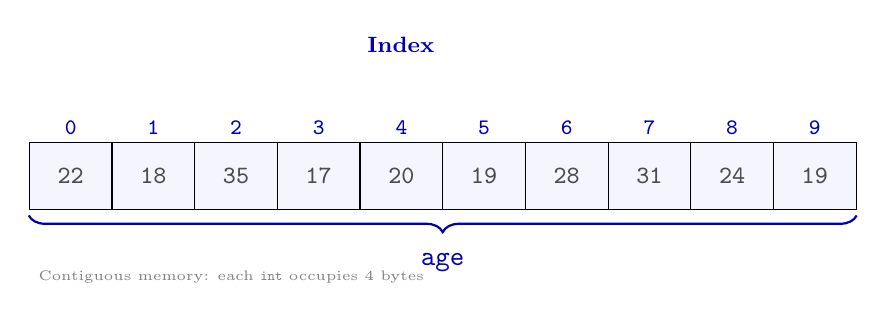
\begin{tikzpicture}[
    cell/.style={
        draw,
        minimum width=1.05cm,
        minimum height=0.85cm,
        anchor=south west,
        font=\small,
        fill=blue!4
    },
    idx/.style={
        font=\footnotesize\ttfamily\bfseries,
        text=blue!70!black
    },
    val/.style={
        font=\small\ttfamily,
        text=black!70
    }
]
% Index heading
\node[font=\footnotesize\bfseries, text=blue!70!black]
    at (4.725, 2.1) {Index};

% Draw cells with index numbers and sample values
\foreach \i/\v in {0/22,1/18,2/35,3/17,4/20,5/19,6/28,7/31,8/24,9/19} {
    \node[cell] (c\i) at (\i*1.05, 0) {};
    % Index on top
    \node[idx] at ([yshift=5pt]c\i.north) {\i};
    % Sample value inside
    \node[val] at (c\i.center) {\v};
}

% Array name brace below
\draw[decorate,
      decoration={brace, amplitude=6pt, mirror},
      thick, blue!70!black]
    ([yshift=-2pt]c0.south west) -- ([yshift=-2pt]c9.south east)
    node[midway, below=10pt, font=\bfseries\ttfamily,
         text=blue!70!black] {age};

% Address hint
\node[font=\tiny, text=gray, anchor=west] at (0, -0.85)
    {Contiguous memory: each \texttt{int} occupies 4 bytes};
\end{tikzpicture}
\end{center}

\begin{infobox}{Memory Layout Detail}
When you declare \texttt{int age[10];}, the compiler allocates
$10 \times \texttt{sizeof(int)} = 10 \times 4 = 40$~bytes of contiguous
memory. The address of element \texttt{age[i]} is
\texttt{base\_address + i\,*\,sizeof(int)}.
This is why array access by index is an $O(1)$ operation.
\end{infobox}

%-----------------------------------------------------------------------------
\section{Initialising Array Elements}
\label{sec:initialising-arrays}
%-----------------------------------------------------------------------------

There are several ways to assign initial values to the elements of an array.

\subsection{Individual Element Initialisation}

Each element can be assigned a value independently:

\begin{cppcode}
age[0] = 18;
age[9] = 19;
\end{cppcode}

\subsection{Initialiser-List Initialisation}

All elements can be initialised at the point of declaration using an
\emph{initialiser list}:

\begin{cppcode}
int age[9] = {18, 17, 18, 18, 19, 20, 17, 18, 19};
\end{cppcode}

\subsection{Auto-Sized Initialisation}

When an initialiser list is provided, the compiler can deduce the size of the
array automatically:

\begin{cppcode}
int x[] = {12, 3, 5, 0, 11, 7, 30, 100, 22};  // size = 9
\end{cppcode}

\subsection{Partial Initialisation with Explicit Size}

If fewer initialisers are provided than the declared size, the remaining
elements are automatically initialised to zero:

\begin{cppcode}
int y[10] = {8, 10, 13, 15, 0, 1, 17, 22};
// y[8] and y[9] are automatically set to 0
\end{cppcode}

\begin{importantbox}{Zero-Initialisation Shortcut}
To set every element of an array to zero, write:
\begin{verbatim}
    int arr[100] = {0};
\end{verbatim}
The first element is explicitly set to \texttt{0}, and the rest are
zero-initialised by the partial-initialisation rule.
\end{importantbox}

The following table summarises all four initialisation methods:

\begin{center}
\renewcommand{\arraystretch}{1.4}
\begin{tabular}{@{} l l @{}}
\toprule
\textbf{Method} & \textbf{Syntax Example} \\
\midrule
Individual assignment & \texttt{age[0] = 18; age[1] = 17;} \\
Full initialiser list & \texttt{int a[3] = \{10, 20, 30\};} \\
Auto-sized            & \texttt{int a[] = \{10, 20, 30\};} \\
Partial (rest = 0)    & \texttt{int a[5] = \{10, 20\};} \\
\bottomrule
\end{tabular}
\end{center}

%-----------------------------------------------------------------------------
\section{Accessing Array Elements}
\label{sec:accessing-arrays}
%-----------------------------------------------------------------------------

Individual elements are accessed by appending the index in square brackets to
the array name. The index of the \emph{first} element is always~\texttt{0};
the index of the \emph{last} element is \texttt{size\,-\,1}.

\begin{cppcode}
int x, y;
x = num[0];   // copy the first element into x
y = num[9];   // copy the tenth element into y
\end{cppcode}

Array elements can participate in any expression, just like ordinary
variables:

\begin{cppcode}
cout << num[0] + num[9];     // print the sum
num[0] = num[1] + num[2];   // assign the sum
num[7] += 3;                 // increment by 3
\end{cppcode}

\begin{warningbox}{Index Out of Bounds}
C++ does \textbf{not} perform automatic bounds checking on array indices. If
you access \texttt{num[10]} in a 10-element array (valid indices 0--9), the
behaviour is \emph{undefined}---your program may crash, produce garbage
values, or corrupt other data.
\end{warningbox}

%-----------------------------------------------------------------------------
\section{Reading, Writing, and Processing Arrays}
\label{sec:rwp-arrays}
%-----------------------------------------------------------------------------

Because arrays work hand-in-hand with loops, nearly all array processing uses
a \texttt{for} loop whose counter variable serves as the index.

\subsection{Writing (Printing) a Single Element}

\begin{cppcode}
cout << num[4];   // print the element at index 4
\end{cppcode}

\subsection{Reading an Array from the User}

\begin{cppcode}
#include <iostream>
using namespace std;

int main() {
    int num[10];

    cout << "Enter 10 integers:" << endl;
    for (int i = 0; i < 10; i++) {
        cin >> num[i];
    }

    return 0;
}
\end{cppcode}

\subsection{Printing an Array in Forward Order}

\begin{cppcode}
cout << "Array elements (forward):" << endl;
for (int i = 0; i < 10; i++) {
    cout << num[i] << " ";
}
cout << endl;
\end{cppcode}

\subsection{Printing an Array in Reverse Order}

\begin{cppcode}
cout << "Array elements (reverse):" << endl;
for (int i = 9; i >= 0; i--) {
    cout << num[i] << " ";
}
cout << endl;
\end{cppcode}

\subsection{Computing the Sum of All Elements}

\begin{cppcode}
int sum = 0;
for (int i = 0; i < 10; i++) {
    sum += num[i];
}
cout << "Sum = " << sum << endl;
\end{cppcode}

%-----------------------------------------------------------------------------
\section{Practical Examples}
\label{sec:array-examples}
%-----------------------------------------------------------------------------

\subsection{Example 1: Accessing Specific Elements}

\textbf{Problem.} Given the array
\texttt{double distance[] = \{23.14, 70.52, 104.08, 468.78, 6.28\}},
display the 2nd and 5th elements.

\begin{cppcode}
#include <iostream>
using namespace std;

int main() {
    double distance[] = {23.14, 70.52, 104.08,
                         468.78, 6.28};

    cout << "2nd element: " << distance[1] << endl;
    cout << "5th element: " << distance[4] << endl;

    return 0;
}
\end{cppcode}

\textbf{Output:}
\begin{verbatim}
2nd element: 70.52
5th element: 6.28
\end{verbatim}

\begin{infobox}{Indexing Starts at Zero}
The ``2nd element'' is at index~1, and the ``5th element'' is at index~4.
Always remember: the $k$-th element is at index $k - 1$.
\end{infobox}

%--------------------------------------------------------------------
\subsection{Example 2: Read and Print in Reverse}

\textbf{Problem.} Read 5 numbers from the user and print them in reverse
order.

\begin{cppcode}
#include <iostream>
using namespace std;

int main() {
    int arr[5];

    cout << "Enter 5 numbers:" << endl;
    for (int i = 0; i < 5; i++) {
        cin >> arr[i];
    }

    cout << "Numbers in reverse order:" << endl;
    for (int i = 4; i >= 0; i--) {
        cout << arr[i] << " ";
    }
    cout << endl;

    return 0;
}
\end{cppcode}

\textbf{Sample run:}
\begin{verbatim}
Enter 5 numbers:
10 20 30 40 50
Numbers in reverse order:
50 40 30 20 10
\end{verbatim}

%--------------------------------------------------------------------
\subsection{Example 3: Summation of Array Elements}

\textbf{Problem.} Read 10 integers into an array and compute their
summation.

\begin{cppcode}
#include <iostream>
using namespace std;

int main() {
    int arr[10];
    int sum = 0;

    cout << "Enter 10 integers:" << endl;
    for (int i = 0; i < 10; i++) {
        cin >> arr[i];
    }

    for (int i = 0; i < 10; i++) {
        sum += arr[i];
    }

    cout << "Summation = " << sum << endl;

    return 0;
}
\end{cppcode}

\textbf{Sample run:}
\begin{verbatim}
Enter 10 integers:
1 2 3 4 5 6 7 8 9 10
Summation = 55
\end{verbatim}

%--------------------------------------------------------------------
\subsection{Example 4: Finding the Minimum Value}

\textbf{Problem.} Read 8 numbers into an array and find the minimum
value.

\begin{cppcode}
#include <iostream>
using namespace std;

int main() {
    int arr[8];

    cout << "Enter 8 numbers:" << endl;
    for (int i = 0; i < 8; i++) {
        cin >> arr[i];
    }

    int min = arr[0];
    for (int i = 1; i < 8; i++) {
        if (arr[i] < min) {
            min = arr[i];
        }
    }

    cout << "Minimum value = " << min << endl;

    return 0;
}
\end{cppcode}

\textbf{Sample run:}
\begin{verbatim}
Enter 8 numbers:
34 12 56 7 89 23 45 11
Minimum value = 7
\end{verbatim}

\begin{infobox}{Finding the Minimum --- Strategy}
\begin{enumerate}
    \item Assume the first element is the minimum.
    \item Compare it with every subsequent element.
    \item Whenever a smaller element is found, update the minimum.
    \item After the loop completes, the variable holds the true
          minimum.
\end{enumerate}
\end{infobox}

%--------------------------------------------------------------------
\subsection{Example 5: Days in Each Month}

\textbf{Problem.} Use an array to store the number of days in each
month (non-leap year) and display them.

\begin{cppcode}
#include <iostream>
using namespace std;

int main() {
    int days[] = {31, 28, 31, 30, 31, 30,
                  31, 31, 30, 31, 30, 31};

    string months[] = {
        "January",   "February", "March",
        "April",     "May",      "June",
        "July",      "August",   "September",
        "October",   "November", "December"
    };

    for (int i = 0; i < 12; i++) {
        cout << months[i] << " has "
             << days[i] << " days." << endl;
    }

    return 0;
}
\end{cppcode}

\textbf{Output (first four lines shown):}
\begin{verbatim}
January has 31 days.
February has 28 days.
March has 31 days.
April has 30 days.
...
\end{verbatim}

\begin{conceptbox}{Parallel Arrays}
Using two arrays of the same size---one for month names and one for day
counts---is called the \textbf{parallel array} technique. The element at
index~\texttt{i} in one array corresponds to the element at the same
index in the other.
\end{conceptbox}

%--------------------------------------------------------------------
\subsection{Example 6: Searching for a Value (Using a Function)}

\textbf{Problem.} Write a function that searches for a value \texttt{X}
in an array and returns its index. If the value is not found,
return~\texttt{-1}.

\begin{cppcode}
#include <iostream>
using namespace std;

int search(int arr[], int size, int x) {
    for (int i = 0; i < size; i++) {
        if (arr[i] == x) {
            return i;   // found: return the index
        }
    }
    return -1;          // not found
}

int main() {
    int arr[] = {10, 25, 33, 47, 52, 68, 71, 89};
    int size = 8;
    int x;

    cout << "Enter a value to search for: ";
    cin >> x;

    int index = search(arr, size, x);

    if (index != -1) {
        cout << x << " found at index "
             << index << endl;
    } else {
        cout << x << " not found in the array."
             << endl;
    }

    return 0;
}
\end{cppcode}

\textbf{Sample run 1:}
\begin{verbatim}
Enter a value to search for: 47
47 found at index 3
\end{verbatim}

\textbf{Sample run 2:}
\begin{verbatim}
Enter a value to search for: 99
99 not found in the array.
\end{verbatim}

\begin{conceptbox}{Linear Search}
The algorithm shown above is called \textbf{linear search} (or
\emph{sequential search}). It examines each element one by one from the
beginning of the array until the target value is found or the end of the
array is reached. Its time complexity is $O(n)$.
\end{conceptbox}

%--------------------------------------------------------------------
\subsection{Example 7: Splitting Odd and Even Numbers}

\textbf{Problem.} Read 10 integers into an array, then split them into
two separate arrays: one for odd numbers and one for even numbers.

\begin{cppcode}
#include <iostream>
using namespace std;

int main() {
    int arr[10];
    int odd[10], even[10];
    int oddCount = 0, evenCount = 0;

    cout << "Enter 10 integers:" << endl;
    for (int i = 0; i < 10; i++) {
        cin >> arr[i];
    }

    for (int i = 0; i < 10; i++) {
        if (arr[i] % 2 == 0) {
            even[evenCount] = arr[i];
            evenCount++;
        } else {
            odd[oddCount] = arr[i];
            oddCount++;
        }
    }

    cout << "Even numbers: ";
    for (int i = 0; i < evenCount; i++) {
        cout << even[i] << " ";
    }
    cout << endl;

    cout << "Odd numbers: ";
    for (int i = 0; i < oddCount; i++) {
        cout << odd[i] << " ";
    }
    cout << endl;

    return 0;
}
\end{cppcode}

\textbf{Sample run:}
\begin{verbatim}
Enter 10 integers:
3 8 15 22 7 40 11 6 9 18
Even numbers: 8 22 40 6 18
Odd numbers: 3 15 7 11 9
\end{verbatim}

\begin{importantbox}{Tracking Array Sizes with Counters}
When the number of elements to be stored in an array is not known in
advance, maintain a separate counter variable (e.g.\ \texttt{oddCount},
\texttt{evenCount}) that tracks how many elements have been inserted so
far. This counter also serves as the index for the next insertion.
\end{importantbox}
    % One-Dimensional Arrays
%=============================================================================
% Chapter 4: Two-Dimensional Arrays
%=============================================================================
\chapter{Two-Dimensional Arrays}
\label{ch:two-dimensional-arrays}

%-----------------------------------------------------------------------------
\section{Introduction to 2D Arrays}
\label{sec:intro-2d-arrays}
%-----------------------------------------------------------------------------

A one-dimensional array stores a single list of values. In many real-world
situations, however, data is naturally organised in a tabular
(row-and-column) format---exam scores for several students across multiple
subjects, pixel intensities in an image, or entries in a mathematical
matrix. For such cases C++ provides \emph{two-dimensional arrays}.

\begin{definitionbox}{Two-Dimensional Array}
A \textbf{two-dimensional (2D) array} is an array of arrays. It is a
collection of elements arranged in rows and columns, where each element is
accessed using \emph{two} indices: a \textbf{row index} and a
\textbf{column index}.
\end{definitionbox}

\begin{conceptbox}{Declaration Syntax}
\begin{verbatim}
    data-type  Array-name[Row-size][Col-size];
\end{verbatim}
\begin{itemize}
    \item \texttt{Row-size} --- the number of rows.
    \item \texttt{Col-size} --- the number of columns.
    \item The total number of elements is
          $\texttt{Row-size} \times \texttt{Col-size}$.
\end{itemize}
\end{conceptbox}

\paragraph{Examples.}

\begin{cppcode}
int a[10][10];   // 10 rows x 10 columns (100 elements)
int num[3][4];   //  3 rows x  4 columns ( 12 elements)
\end{cppcode}

\subsection*{Visualising a 2D Array}

The diagram below shows the layout of \texttt{int num[3][4]}. Rows are
numbered 0--2 and columns 0--3.

\begin{center}
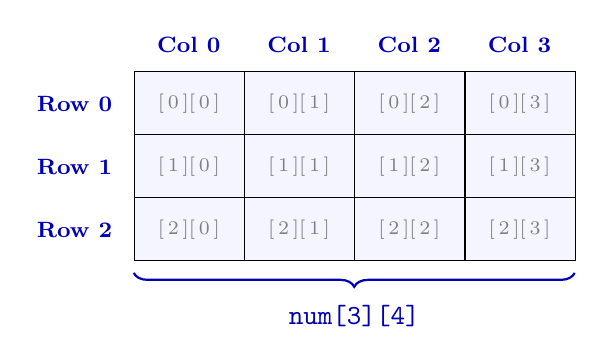
\begin{tikzpicture}[
    cell/.style={
        draw,
        minimum width=1.4cm,
        minimum height=0.8cm,
        anchor=south west,
        font=\small\ttfamily,
        fill=blue!4
    },
    hdr/.style={
        font=\footnotesize\bfseries,
        text=blue!70!black
    }
]
% Column headers
\foreach \j in {0,...,3} {
    \node[hdr] at (\j*1.4+0.7, 2.75) {Col \j};
}

% Row 2 (index 0 at top of diagram)
\node[hdr, anchor=east] at (-0.15, 2.0) {Row 0};
\foreach \j in {0,...,3} {
    \node[cell] at (\j*1.4, 1.6) {};
    \node[font=\scriptsize, gray] at (\j*1.4+0.7, 2.0) {[\,0\,][\,\j\,]};
}

% Row 1
\node[hdr, anchor=east] at (-0.15, 1.2) {Row 1};
\foreach \j in {0,...,3} {
    \node[cell] at (\j*1.4, 0.8) {};
    \node[font=\scriptsize, gray] at (\j*1.4+0.7, 1.2) {[\,1\,][\,\j\,]};
}

% Row 0
\node[hdr, anchor=east] at (-0.15, 0.4) {Row 2};
\foreach \j in {0,...,3} {
    \node[cell] at (\j*1.4, 0) {};
    \node[font=\scriptsize, gray] at (\j*1.4+0.7, 0.4) {[\,2\,][\,\j\,]};
}

% Array name brace
\draw[decorate,
      decoration={brace, amplitude=5pt, mirror},
      thick, blue!70!black]
    (0, -0.15) -- (5.6, -0.15)
    node[midway, below=8pt, font=\bfseries\ttfamily,
         text=blue!70!black] {num[3][4]};
\end{tikzpicture}
\end{center}

\begin{infobox}{Memory Layout}
Although we visualise a 2D array as a grid, in memory the elements are
stored in \emph{row-major order}: all elements of row~0 come first,
followed by all elements of row~1, and so on.

\medskip
\begin{center}
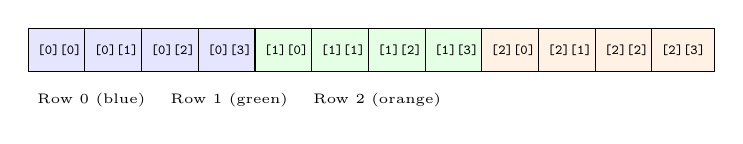
\begin{tikzpicture}[
    cell/.style={
        draw, minimum width=0.72cm, minimum height=0.55cm,
        font=\tiny\ttfamily, fill=white, anchor=south west
    }
]
\foreach \i/\lbl/\clr in {%
    0/{[0][0]}/blue!10, 1/{[0][1]}/blue!10,
    2/{[0][2]}/blue!10, 3/{[0][3]}/blue!10,
    4/{[1][0]}/green!10, 5/{[1][1]}/green!10,
    6/{[1][2]}/green!10, 7/{[1][3]}/green!10,
    8/{[2][0]}/orange!10, 9/{[2][1]}/orange!10,
    10/{[2][2]}/orange!10, 11/{[2][3]}/orange!10%
} {
    \node[cell, fill=\clr] at (\i*0.72, 0) {\lbl};
}
\node[font=\tiny, anchor=west] at (0, -0.35)
    {Row 0 (blue) \quad Row 1 (green) \quad Row 2 (orange)};
\end{tikzpicture}
\end{center}
\end{infobox}

%-----------------------------------------------------------------------------
\section{Initialising 2D Arrays}
\label{sec:init-2d-arrays}
%-----------------------------------------------------------------------------

A two-dimensional array can be initialised at the point of declaration using
nested brace-enclosed lists---one inner list per row:

\begin{cppcode}
int a[2][3] = {
    {1, 2, 3},   // row 0
    {4, 5, 6}    // row 1
};
\end{cppcode}

\subsection*{Resulting Layout}

The table below shows the values stored in each position after the
initialisation above.

\begin{center}
\renewcommand{\arraystretch}{1.3}
\begin{tabular}{@{} c ccc @{}}
\toprule
    & \textbf{Col 0} & \textbf{Col 1} & \textbf{Col 2} \\
\midrule
\textbf{Row 0} & 1 & 2 & 3 \\
\textbf{Row 1} & 4 & 5 & 6 \\
\bottomrule
\end{tabular}
\end{center}

\begin{warningbox}{Row Size Can Be Omitted --- Column Size Cannot}
When an initialiser list is provided, the compiler can deduce the number
of rows, so you may write
\texttt{int a[][3] = \{\{1,2,3\},\{4,5,6\}\};}. However, the
\emph{column} size must always be specified explicitly.
\end{warningbox}

%-----------------------------------------------------------------------------
\section{Reading, Writing, and Processing 2D Arrays}
\label{sec:rwp-2d-arrays}
%-----------------------------------------------------------------------------

Processing a 2D array requires \emph{nested loops}: the outer loop iterates
over the rows, and the inner loop iterates over the columns (or vice versa).

%--------------------------------------------------------------------
\subsection{Example 1: Read and Print a
            3\texorpdfstring{\texttimes}{x}5 Array}

\textbf{Problem.} Read a $3 \times 5$ array of integers from the user,
then print all elements.

\begin{cppcode}
#include <iostream>
using namespace std;

int main() {
    int arr[3][5];

    // Reading
    cout << "Enter 15 integers (3 rows x 5 cols):"
         << endl;
    for (int i = 0; i < 3; i++) {
        for (int j = 0; j < 5; j++) {
            cin >> arr[i][j];
        }
    }

    // Printing
    cout << "Array elements:" << endl;
    for (int i = 0; i < 3; i++) {
        for (int j = 0; j < 5; j++) {
            cout << arr[i][j] << "\t";
        }
        cout << endl;
    }

    return 0;
}
\end{cppcode}

\textbf{Sample run:}
\begin{verbatim}
Enter 15 integers (3 rows x 5 cols):
1 2 3 4 5 6 7 8 9 10 11 12 13 14 15
Array elements:
1       2       3       4       5
6       7       8       9       10
11      12      13      14      15
\end{verbatim}

%--------------------------------------------------------------------
\subsection{Example 2: Read, Sum, and Print a
            4\texorpdfstring{\texttimes}{x}4 Array}

\textbf{Problem.} Read a $4 \times 4$ array, compute the summation of
all elements, and print the array together with the total.

\begin{cppcode}
#include <iostream>
using namespace std;

int main() {
    int arr[4][4];
    int sum = 0;

    cout << "Enter 16 integers (4 x 4):" << endl;
    for (int i = 0; i < 4; i++) {
        for (int j = 0; j < 4; j++) {
            cin >> arr[i][j];
        }
    }

    // Print and accumulate
    cout << "Array elements:" << endl;
    for (int i = 0; i < 4; i++) {
        for (int j = 0; j < 4; j++) {
            cout << arr[i][j] << "\t";
            sum += arr[i][j];
        }
        cout << endl;
    }

    cout << "Summation of all elements = "
         << sum << endl;

    return 0;
}
\end{cppcode}

\textbf{Sample run:}
\begin{verbatim}
Enter 16 integers (4 x 4):
1 2 3 4 5 6 7 8 9 10 11 12 13 14 15 16
Array elements:
1       2       3       4
5       6       7       8
9       10      11      12
13      14      15      16
Summation of all elements = 136
\end{verbatim}

%--------------------------------------------------------------------
\subsection{Example 3: Summation of Each Row}

\textbf{Problem.} Read a $3 \times 4$ array and compute the summation
of each row separately.

\begin{cppcode}
#include <iostream>
using namespace std;

int main() {
    int arr[3][4];

    cout << "Enter 12 integers (3 x 4):" << endl;
    for (int i = 0; i < 3; i++) {
        for (int j = 0; j < 4; j++) {
            cin >> arr[i][j];
        }
    }

    for (int i = 0; i < 3; i++) {
        int rowSum = 0;
        for (int j = 0; j < 4; j++) {
            rowSum += arr[i][j];
        }
        cout << "Sum of row " << i
             << " = " << rowSum << endl;
    }

    return 0;
}
\end{cppcode}

\textbf{Sample run:}
\begin{verbatim}
Enter 12 integers (3 x 4):
1 2 3 4 5 6 7 8 9 10 11 12
Sum of row 0 = 10
Sum of row 1 = 26
Sum of row 2 = 42
\end{verbatim}

\begin{importantbox}{Row Summation Pattern}
To sum each row independently, reset the accumulator variable
(\texttt{rowSum}) to zero at the \emph{beginning} of each iteration of
the outer loop. This ensures that each row's total is computed from
scratch.
\end{importantbox}

%--------------------------------------------------------------------
\subsection{Example 4: Replace a Specific Value}

\textbf{Problem.} Read a $3 \times 4$ array and replace every
occurrence of the value~5 with~0.

\begin{cppcode}
#include <iostream>
using namespace std;

int main() {
    int arr[3][4];

    cout << "Enter 12 integers (3 x 4):" << endl;
    for (int i = 0; i < 3; i++) {
        for (int j = 0; j < 4; j++) {
            cin >> arr[i][j];
        }
    }

    // Replace 5 with 0
    for (int i = 0; i < 3; i++) {
        for (int j = 0; j < 4; j++) {
            if (arr[i][j] == 5) {
                arr[i][j] = 0;
            }
        }
    }

    // Print the modified array
    cout << "Array after replacement:" << endl;
    for (int i = 0; i < 3; i++) {
        for (int j = 0; j < 4; j++) {
            cout << arr[i][j] << "\t";
        }
        cout << endl;
    }

    return 0;
}
\end{cppcode}

\textbf{Sample run:}
\begin{verbatim}
Enter 12 integers (3 x 4):
1 5 3 4 5 6 5 8 9 10 5 12
Array after replacement:
1       0       3       4
0       6       0       8
9       10      0       12
\end{verbatim}

%--------------------------------------------------------------------
\subsection{Example 5: Adding Two 2D Arrays}

\textbf{Problem.} Read two $3 \times 4$ arrays and compute their
element-wise sum into a third array.

\begin{cppcode}
#include <iostream>
using namespace std;

int main() {
    int a[3][4], b[3][4], c[3][4];

    cout << "Enter first array (3 x 4):" << endl;
    for (int i = 0; i < 3; i++)
        for (int j = 0; j < 4; j++)
            cin >> a[i][j];

    cout << "Enter second array (3 x 4):" << endl;
    for (int i = 0; i < 3; i++)
        for (int j = 0; j < 4; j++)
            cin >> b[i][j];

    // Element-wise addition
    for (int i = 0; i < 3; i++)
        for (int j = 0; j < 4; j++)
            c[i][j] = a[i][j] + b[i][j];

    // Print the result
    cout << "Sum of the two arrays:" << endl;
    for (int i = 0; i < 3; i++) {
        for (int j = 0; j < 4; j++) {
            cout << c[i][j] << "\t";
        }
        cout << endl;
    }

    return 0;
}
\end{cppcode}

\textbf{Sample run:}
\begin{verbatim}
Enter first array (3 x 4):
1 2 3 4 5 6 7 8 9 10 11 12
Enter second array (3 x 4):
10 20 30 40 50 60 70 80 90 100 110 120
Sum of the two arrays:
11      22      33      44
55      66      77      88
99      110     121     132
\end{verbatim}

%--------------------------------------------------------------------
\subsection{Example 6: Converting a 2D Array to a 1D Array}

\textbf{Problem.} Given a $3 \times 4$ array, copy all of its elements
into a one-dimensional array of size~12.

\begin{cppcode}
#include <iostream>
using namespace std;

int main() {
    int arr2D[3][4];
    int arr1D[12];

    cout << "Enter 12 integers (3 x 4):" << endl;
    for (int i = 0; i < 3; i++)
        for (int j = 0; j < 4; j++)
            cin >> arr2D[i][j];

    // Flatten 2D -> 1D
    int k = 0;
    for (int i = 0; i < 3; i++) {
        for (int j = 0; j < 4; j++) {
            arr1D[k] = arr2D[i][j];
            k++;
        }
    }

    // Print the 1D array
    cout << "1D array: ";
    for (int i = 0; i < 12; i++) {
        cout << arr1D[i] << " ";
    }
    cout << endl;

    return 0;
}
\end{cppcode}

\textbf{Sample run:}
\begin{verbatim}
Enter 12 integers (3 x 4):
1 2 3 4 5 6 7 8 9 10 11 12
1D array: 1 2 3 4 5 6 7 8 9 10 11 12
\end{verbatim}

\begin{conceptbox}{Flattening a 2D Array}
Converting a 2D array with $R$ rows and $C$ columns into a 1D array of
size $R \times C$ is called \textbf{flattening}. The element at position
\texttt{[i][j]} in the 2D array maps to index $i \times C + j$ in the
1D array. Equivalently, you can use a simple counter variable \texttt{k}
that increments with every element, as shown above.
\end{conceptbox}

%-----------------------------------------------------------------------------
\section{Matrix Diagonal Operations}
\label{sec:diagonal-operations}
%-----------------------------------------------------------------------------

When a 2D array represents a square matrix (same number of rows and
columns), several special index relationships identify important regions
of the matrix.

\begin{definitionbox}{Diagonal and Triangular Regions}
For an $n \times n$ square matrix with row index $i$ and column index $j$
(both starting from~0):
\begin{itemize}
    \item \textbf{Main diagonal:} elements where $i = j$.
    \item \textbf{Secondary diagonal:} elements where
          $i + j = n - 1$.
    \item \textbf{Upper triangle:} elements where $i < j$
          (above the main diagonal).
    \item \textbf{Lower triangle:} elements where $i > j$
          (below the main diagonal).
\end{itemize}
\end{definitionbox}

\subsection*{Visual Reference --- 3\texorpdfstring{\texttimes}{x}3
             Matrix}

The following colour-coded diagram illustrates these regions for a
$3 \times 3$ matrix. Each cell shows the index condition it satisfies.

\begin{center}
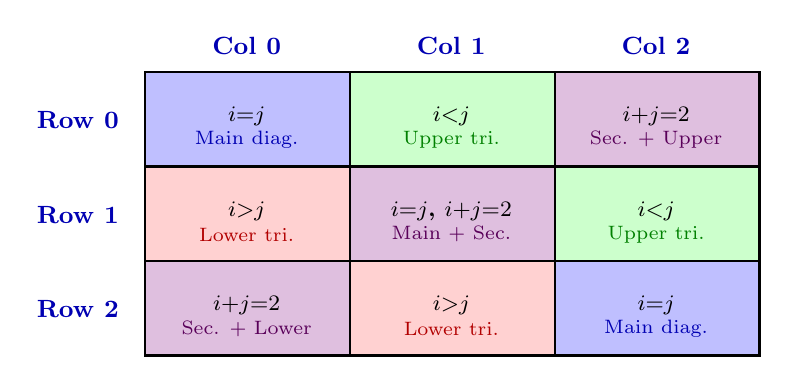
\begin{tikzpicture}[
    cell/.style={
        draw, thick,
        minimum width=2.6cm,
        minimum height=1.2cm,
        anchor=south west,
        font=\small
    },
    main/.style={cell, fill=blue!25},
    secondary/.style={cell, fill=orange!35},
    upper/.style={cell, fill=green!20},
    lower/.style={cell, fill=red!18},
    both/.style={cell, fill=violet!25},
    hdr/.style={font=\small\bfseries, text=blue!70!black}
]
% Column headers
\foreach \j in {0,1,2} {
    \node[hdr] at (\j*2.6+1.3, 3.95) {Col \j};
}

% ------- Row 0 (top, y=2.4) -------
\node[hdr, anchor=east] at (-0.2, 3.0) {Row 0};
% (0,0): i==j => Main diagonal
\node[main] at (0, 2.4) {};
\node[font=\footnotesize\bfseries] at (1.3, 3.05) {$i{=}j$};
\node[font=\scriptsize, text=blue!70!black] at (1.3, 2.75)
    {Main diag.};

% (0,1): i<j => Upper triangle
\node[upper] at (2.6, 2.4) {};
\node[font=\footnotesize\bfseries] at (3.9, 3.05) {$i{<}j$};
\node[font=\scriptsize, text=green!50!black] at (3.9, 2.75)
    {Upper tri.};

% (0,2): i<j AND i+j==2 => Secondary + Upper
\node[both] at (5.2, 2.4) {};
\node[font=\footnotesize\bfseries] at (6.5, 3.05)
    {$i{+}j{=}2$};
\node[font=\scriptsize, text=violet!70!black] at (6.5, 2.75)
    {Sec. + Upper};

% ------- Row 1 (middle, y=1.2) -------
\node[hdr, anchor=east] at (-0.2, 1.8) {Row 1};
% (1,0): i>j => Lower triangle
\node[lower] at (0, 1.2) {};
\node[font=\footnotesize\bfseries] at (1.3, 1.85) {$i{>}j$};
\node[font=\scriptsize, text=red!70!black] at (1.3, 1.55)
    {Lower tri.};

% (1,1): i==j AND i+j==2 => Main + Secondary
\node[both] at (2.6, 1.2) {};
\node[font=\footnotesize\bfseries] at (3.9, 1.85)
    {$i{=}j$, $i{+}j{=}2$};
\node[font=\scriptsize, text=violet!70!black] at (3.9, 1.55)
    {Main + Sec.};

% (1,2): i<j => Upper triangle
\node[upper] at (5.2, 1.2) {};
\node[font=\footnotesize\bfseries] at (6.5, 1.85) {$i{<}j$};
\node[font=\scriptsize, text=green!50!black] at (6.5, 1.55)
    {Upper tri.};

% ------- Row 2 (bottom, y=0) -------
\node[hdr, anchor=east] at (-0.2, 0.6) {Row 2};
% (2,0): i>j AND i+j==2 => Secondary + Lower
\node[both] at (0, 0) {};
\node[font=\footnotesize\bfseries] at (1.3, 0.65)
    {$i{+}j{=}2$};
\node[font=\scriptsize, text=violet!70!black] at (1.3, 0.35)
    {Sec. + Lower};

% (2,1): i>j => Lower triangle
\node[lower] at (2.6, 0) {};
\node[font=\footnotesize\bfseries] at (3.9, 0.65) {$i{>}j$};
\node[font=\scriptsize, text=red!70!black] at (3.9, 0.35)
    {Lower tri.};

% (2,2): i==j => Main diagonal
\node[main] at (5.2, 0) {};
\node[font=\footnotesize\bfseries] at (6.5, 0.65) {$i{=}j$};
\node[font=\scriptsize, text=blue!70!black] at (6.5, 0.35)
    {Main diag.};
\end{tikzpicture}
\end{center}

\medskip

% Legend as a compact table
\begin{center}
\renewcommand{\arraystretch}{1.2}
\begin{tabular}{@{} >{\centering\arraybackslash}p{1.8cm}
                    >{\centering\arraybackslash}p{1.8cm}
                    >{\centering\arraybackslash}p{1.8cm}
                    >{\centering\arraybackslash}p{1.8cm}
                    >{\centering\arraybackslash}p{1.8cm} @{}}
\toprule
\colorbox{blue!25}{\strut\hspace{8mm}} &
\colorbox{orange!35}{\strut\hspace{8mm}} &
\colorbox{green!20}{\strut\hspace{8mm}} &
\colorbox{red!18}{\strut\hspace{8mm}} &
\colorbox{violet!25}{\strut\hspace{8mm}} \\
\footnotesize Main diag. &
\footnotesize Sec.\ diag. &
\footnotesize Upper tri. &
\footnotesize Lower tri. &
\footnotesize Overlap \\
\footnotesize $i = j$ &
\footnotesize $i{+}j = n{-}1$ &
\footnotesize $i < j$ &
\footnotesize $i > j$ &
\footnotesize (both) \\
\bottomrule
\end{tabular}
\end{center}

\medskip

The following summary table also maps every cell of a $3\times 3$ matrix
to its region:

\begin{center}
\renewcommand{\arraystretch}{1.3}
\begin{tabular}{@{} c ccc @{}}
\toprule
    & \textbf{Col 0} & \textbf{Col 1} & \textbf{Col 2} \\
\midrule
\textbf{Row 0}
    & $a_{00}$\;\textsuperscript{main}
    & $a_{01}$\;\textsuperscript{upper}
    & $a_{02}$\;\textsuperscript{sec., upper} \\
\textbf{Row 1}
    & $a_{10}$\;\textsuperscript{lower}
    & $a_{11}$\;\textsuperscript{main, sec.}
    & $a_{12}$\;\textsuperscript{upper} \\
\textbf{Row 2}
    & $a_{20}$\;\textsuperscript{sec., lower}
    & $a_{21}$\;\textsuperscript{lower}
    & $a_{22}$\;\textsuperscript{main} \\
\bottomrule
\end{tabular}
\end{center}

%--------------------------------------------------------------------
\subsection{Example 7: Replace Main Diagonal with Zero}

\textbf{Problem.} Read a $4 \times 4$ matrix and replace all elements
on the main diagonal with zero, then print the result.

\begin{cppcode}
#include <iostream>
using namespace std;

int main() {
    int arr[4][4];

    cout << "Enter 16 integers (4 x 4):" << endl;
    for (int i = 0; i < 4; i++)
        for (int j = 0; j < 4; j++)
            cin >> arr[i][j];

    // Replace main diagonal elements with 0
    for (int i = 0; i < 4; i++) {
        arr[i][i] = 0;   // main diagonal: i == j
    }

    // Print the modified matrix
    cout << "Matrix after replacing diagonal:"
         << endl;
    for (int i = 0; i < 4; i++) {
        for (int j = 0; j < 4; j++) {
            cout << arr[i][j] << "\t";
        }
        cout << endl;
    }

    return 0;
}
\end{cppcode}

\textbf{Sample run:}
\begin{verbatim}
Enter 16 integers (4 x 4):
1 2 3 4 5 6 7 8 9 10 11 12 13 14 15 16
Matrix after replacing diagonal:
0       2       3       4
5       0       7       8
9       10      0       12
13      14      15      0
\end{verbatim}

\begin{infobox}{Accessing the Main Diagonal Efficiently}
Since main-diagonal elements satisfy $i = j$, you only need a
\emph{single} loop---not nested loops---to visit them all:
\texttt{for (int i = 0; i < n; i++) arr[i][i] = 0;}.
\end{infobox}

%--------------------------------------------------------------------
\subsection{Example 8: Square Root of Array Elements}

\textbf{Problem.} Read a $3 \times 3$ array of \texttt{double} values
and print the square root of each element.

\begin{cppcode}
#include <iostream>
#include <cmath>
using namespace std;

int main() {
    double arr[3][3];

    cout << "Enter 9 values (3 x 3):" << endl;
    for (int i = 0; i < 3; i++)
        for (int j = 0; j < 3; j++)
            cin >> arr[i][j];

    cout << "Square roots:" << endl;
    for (int i = 0; i < 3; i++) {
        for (int j = 0; j < 3; j++) {
            cout << sqrt(arr[i][j]) << "\t";
        }
        cout << endl;
    }

    return 0;
}
\end{cppcode}

\textbf{Sample run:}
\begin{verbatim}
Enter 9 values (3 x 3):
4 9 16 25 36 49 64 81 100
Square roots:
2       3       4
5       6       7
8       9       10
\end{verbatim}

\begin{warningbox}{Negative Values under \texttt{sqrt}}
The \texttt{sqrt} function from \texttt{<cmath>} returns \texttt{NaN}
(Not a Number) when given a negative argument. In a robust program you
should validate that each value is non-negative before computing its
square root.
\end{warningbox}

%--------------------------------------------------------------------
\subsection{Example 9: Sum of Main and Secondary Diagonals}

\textbf{Problem.} Read a $4 \times 4$ integer matrix and compute:
\begin{enumerate}
    \item The sum of the \emph{main diagonal} elements.
    \item The sum of the \emph{secondary diagonal} elements.
\end{enumerate}

\begin{cppcode}
#include <iostream>
using namespace std;

int main() {
    int arr[4][4];
    int mainSum = 0, secSum = 0;
    int n = 4;

    cout << "Enter 16 integers (4 x 4):" << endl;
    for (int i = 0; i < n; i++)
        for (int j = 0; j < n; j++)
            cin >> arr[i][j];

    for (int i = 0; i < n; i++) {
        mainSum += arr[i][i];
        secSum  += arr[i][n - 1 - i];
    }

    cout << "Sum of main diagonal      = "
         << mainSum << endl;
    cout << "Sum of secondary diagonal  = "
         << secSum  << endl;

    return 0;
}
\end{cppcode}

\textbf{Sample run:}
\begin{verbatim}
Enter 16 integers (4 x 4):
1 2 3 4 5 6 7 8 9 10 11 12 13 14 15 16
Sum of main diagonal      = 34
Sum of secondary diagonal  = 34
\end{verbatim}

\begin{importantbox}{Diagonal Summation in a Single Loop}
Both diagonal sums can be computed in a single loop of $n$ iterations.
\begin{itemize}
    \item For the main diagonal, the column index equals the row
          index: use \texttt{arr[i][i]}.
    \item For the secondary diagonal, the column index is
          \texttt{n\,-\,1\,-\,i}: use \texttt{arr[i][n-1-i]}.
\end{itemize}
Note: in a matrix with an odd dimension, the centre element belongs to
\emph{both} diagonals. If you need the combined sum without
double-counting, subtract that centre element once.
\end{importantbox}
    % Two-Dimensional Arrays
%=============================================================================
% Chapter 5: Strings in C++
%=============================================================================
\chapter{Strings in C++}
\label{ch:strings}

%-----------------------------------------------------------------------------
\section{Introduction to Strings}
\label{sec:strings-intro}
%-----------------------------------------------------------------------------

\begin{definitionbox}{C-Style Strings}
In C++ strings of characters are implemented as an array of characters
with a \textbf{null terminator} \texttt{'\textbackslash 0'}.  The null
character marks the end of the string so that library functions know where
the string data stops.
\end{definitionbox}

\noindent
The general form for declaring a character string is:

\begin{cppcode}
char String_name[size];
\end{cppcode}

\noindent
where \texttt{size} specifies the maximum number of characters the array
can hold, \emph{including} the null terminator.

\subsection{Initialising Strings}

A string can be initialised at declaration time in several ways:

\begin{cppcode}
char name[11] = "Mazin Alaa";   // size must include '\0'
char str[]    = "ABCD";         // compiler sets size = 5
\end{cppcode}

\begin{warningbox}{Size Must Include the Null Terminator}
When you specify the size explicitly, remember to count the
\texttt{'\textbackslash 0'} character.  For example,
\texttt{"Mazin Alaa"} has 10 visible characters, so the array must be
at least \texttt{[11]}.
\end{warningbox}

\subsection{Character-by-Character Storage}

When the compiler stores \texttt{str[] = "ABCD"}, the memory layout is
as follows:

\begin{center}
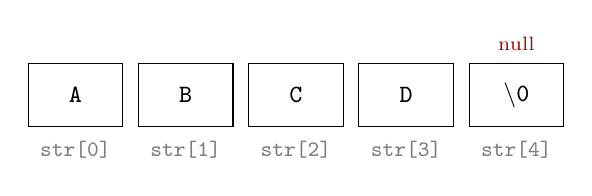
\begin{tikzpicture}[
    cell/.style={draw, minimum width=1.2cm, minimum height=0.8cm,
                 font=\ttfamily\small},
    label/.style={font=\footnotesize\ttfamily, text=gray}
]
  \foreach \c/\i in {A/0, B/1, C/2, D/3, \textbackslash 0/4} {
    \node[cell] (c\i) at (\i*1.4, 0) {\c};
    \node[label] at (\i*1.4, -0.7) {str[\i]};
  }
  \node[font=\scriptsize, text=red!70!black] at (4*1.4, 0.65)
       {null};
\end{tikzpicture}
\end{center}

\begin{importantbox}{The Null Terminator}
The character \texttt{'\textbackslash 0'} (ASCII value 0) is
automatically appended by the compiler when you use a string literal.
Without it, functions such as \texttt{cout}, \texttt{strlen}, and
\texttt{strcpy} will read past the intended boundary, causing
undefined behaviour.
\end{importantbox}

%-----------------------------------------------------------------------------
\section{Reading, Writing, and Processing Strings}
\label{sec:strings-rw}
%-----------------------------------------------------------------------------

\subsection{Example 1 --- Printing a String}

The following program prints an entire string and then prints it
character by character using a loop:

\begin{cppcode}
#include <iostream>
using namespace std;

int main() {
    char str[] = "Hello, World!";

    // Print the whole string at once
    cout << "Full string: " << str << endl;

    // Print character by character
    cout << "Char by char: ";
    for (int i = 0; str[i] != '\0'; i++) {
        cout << str[i];
    }
    cout << endl;

    return 0;
}
\end{cppcode}

\noindent
\textbf{Sample run:}
\begin{verbatim}
Full string: Hello, World!
Char by char: Hello, World!
\end{verbatim}

\begin{conceptbox}{Iterating Over a C-String}
The idiomatic way to walk through a C-string is to loop while
\texttt{str[i] != '\textbackslash 0'}.  This works because every
properly formed C-string is guaranteed to end with the null character.
\end{conceptbox}

\subsection{Example 2 --- Converting Lowercase to Uppercase}

The library function \texttt{toupper()} (declared in
\texttt{<cctype>}) converts a single lowercase letter to its uppercase
equivalent.  Non-lowercase characters are returned unchanged.

\begin{cppcode}
#include <iostream>
#include <cctype>
using namespace std;

int main() {
    char str[50];

    cout << "Enter a string: ";
    cin.getline(str, 50);

    for (int i = 0; str[i] != '\0'; i++) {
        str[i] = toupper(str[i]);
    }

    cout << "Uppercase: " << str << endl;

    return 0;
}
\end{cppcode}

\noindent
\textbf{Sample run:}
\begin{verbatim}
Enter a string: Hello World
Uppercase: HELLO WORLD
\end{verbatim}

%-----------------------------------------------------------------------------
\section{String I/O Functions}
\label{sec:strings-io}
%-----------------------------------------------------------------------------

\begin{infobox}{Useful String I/O Functions}
\begin{tabular}{@{}l l@{}}
\texttt{cin.getline(str, n);} & Read up to \texttt{n-1} characters
    (including spaces) into \texttt{str}. \\[4pt]
\texttt{cin.get(ch);}         & Read a single character (including
    whitespace) into \texttt{ch}. \\[4pt]
\texttt{cin.ignore(n, delim);} & Discard up to \texttt{n} characters
    or until \texttt{delim} is found. \\[4pt]
\texttt{cin.putback(ch);}     & Push character \texttt{ch} back into
    the input buffer. \\[4pt]
\texttt{cout.put(ch);}        & Write a single character to standard
    output. \\
\end{tabular}
\end{infobox}

\begin{cppcode}
#include <iostream>
using namespace std;

int main() {
    char line[80], ch;

    cout << "Enter a line: ";
    cin.getline(line, 80);       // reads full line with spaces
    cout << "You entered: " << line << endl;

    cout << "Enter a character: ";
    cin.get(ch);                 // reads one character
    cout << "Character: ";
    cout.put(ch);                // writes one character
    cout << endl;

    cin.ignore(80, '\n');        // flush remaining input

    return 0;
}
\end{cppcode}

\noindent
\textbf{Sample run:}
\begin{verbatim}
Enter a line: Programming is fun
You entered: Programming is fun
Enter a character: X
Character: X
\end{verbatim}

\begin{warningbox}{\texttt{cin >>} vs.\ \texttt{cin.getline()}}
The extraction operator \texttt{>>} stops reading at the first
whitespace character, so it cannot read a full sentence.  Use
\texttt{cin.getline()} when you need to capture an entire line
including spaces.
\end{warningbox}

%-----------------------------------------------------------------------------
\section{String Library Functions (\texttt{string.h})}
\label{sec:string-lib}
%-----------------------------------------------------------------------------

The header \texttt{<cstring>} (or the older \texttt{<string.h>})
provides a rich set of functions for manipulating C-style strings.
Table~\ref{tab:string-funcs} summarises the most commonly used ones.

\begin{table}[htbp]
\centering
\caption{Common \texttt{<cstring>} library functions.}
\label{tab:string-funcs}
\renewcommand{\arraystretch}{1.4}
\begin{tabular}{@{} l p{4.8cm} p{5.5cm} @{}}
\toprule
\textbf{Function} & \textbf{Description} & \textbf{Example} \\
\midrule
\texttt{strlen(s)} &
    Returns the number of characters in \texttt{s}, \emph{excluding}
    the null terminator. &
    \texttt{char a[]="abcd";}\newline
    \texttt{cout << strlen(a);}\newline
    \textit{Output:} \texttt{4} \\
\addlinespace
\texttt{strcpy(dest, src)} &
    Copies the string \texttt{src} (including \texttt{'\textbackslash 0'})
    into \texttt{dest}. &
    \texttt{char a[]="abcd", b[10];}\newline
    \texttt{strcpy(b, a);}\newline
    \textit{b is now} \texttt{"abcd"} \\
\addlinespace
\texttt{strcat(s1, s2)} &
    Appends a copy of \texttt{s2} to the end of \texttt{s1}.
    \texttt{s1} must have enough room. &
    \texttt{char a[20]="abcd";}\newline
    \texttt{char b[]="1234";}\newline
    \texttt{strcat(a, b);}\newline
    \textit{a is now} \texttt{"abcd1234"} \\
\addlinespace
\texttt{strcmp(s1, s2)} &
    Compares two strings lexicographically.\newline
    Returns \texttt{0} if equal, a positive value if
    \texttt{s1 > s2}, a negative value if \texttt{s1 < s2}. &
    \texttt{strcmp("abc","abc");} $\rightarrow$ \texttt{0}\newline
    \texttt{strcmp("b","a");}\ \ $\rightarrow$ \texttt{+}\newline
    \texttt{strcmp("a","b");}\ \ $\rightarrow$ \texttt{-} \\
\bottomrule
\end{tabular}
\end{table}

\begin{cppcode}
#include <iostream>
#include <cstring>
using namespace std;

int main() {
    char s1[30] = "Hello";
    char s2[]   = " World";

    cout << "Length of s1: " << strlen(s1) << endl;   // 5

    strcat(s1, s2);
    cout << "After strcat: " << s1 << endl;           // Hello World

    char s3[30];
    strcpy(s3, s1);
    cout << "Copied s3:    " << s3 << endl;           // Hello World

    if (strcmp(s1, s3) == 0)
        cout << "s1 and s3 are equal." << endl;

    return 0;
}
\end{cppcode}

\noindent
\textbf{Sample run:}
\begin{verbatim}
Length of s1: 5
After strcat: Hello World
Copied s3:    Hello World
s1 and s3 are equal.
\end{verbatim}

\begin{warningbox}{Buffer Overflow with C-Strings}
C-style string functions such as \texttt{strcpy()} and \texttt{strcat()}
do \emph{not} check whether the destination array is large enough.
Writing past the end of the array causes a \textbf{buffer overflow},
which can corrupt other variables, crash the program, or create
security vulnerabilities.  Always ensure the destination has
enough room, including the null terminator.
\end{warningbox}

%-----------------------------------------------------------------------------
\section{\texttt{stdlib} Library Functions}
\label{sec:stdlib-funcs}
%-----------------------------------------------------------------------------

The header \texttt{<cstdlib>} provides functions for converting between
strings and numeric types.  Table~\ref{tab:stdlib-funcs} lists the most
important ones.

\begin{table}[htbp]
\centering
\caption{Common \texttt{<cstdlib>} conversion functions.}
\label{tab:stdlib-funcs}
\renewcommand{\arraystretch}{1.4}
\begin{tabular}{@{} l p{4.5cm} p{5.8cm} @{}}
\toprule
\textbf{Function} & \textbf{Description} & \textbf{Example} \\
\midrule
\texttt{atoi(s)} &
    Converts the string \texttt{s} to an \texttt{int}. &
    \texttt{char a[]="1234";}\newline
    \texttt{int i = atoi(a);}\newline
    \textit{i is now} \texttt{1234} \\
\addlinespace
\texttt{atof(s)} &
    Converts the string \texttt{s} to a \texttt{double}. &
    \texttt{char a[]="12.34";}\newline
    \texttt{double f = atof(a);}\newline
    \textit{f is now} \texttt{12.34} \\
\addlinespace
\texttt{itoa(i, s, base)} &
    Converts the integer \texttt{i} to a string stored in \texttt{s}
    using the specified \texttt{base} (e.g.\ 10 for decimal). &
    \texttt{int i = 1234;}\newline
    \texttt{char a[10];}\newline
    \texttt{itoa(i, a, 10);}\newline
    \textit{a is now} \texttt{"1234"} \\
\bottomrule
\end{tabular}
\end{table}

\begin{warningbox}{\texttt{itoa} is Non-Standard}
The function \texttt{itoa()} is not part of the C++ standard; it is a
compiler extension available in some implementations (e.g.\ older
Borland and MSVC compilers).  For portable code, prefer
\texttt{sprintf()} or \texttt{std::to\_string()} (C++11).
\end{warningbox}

\begin{cppcode}
#include <iostream>
#include <cstdlib>
using namespace std;

int main() {
    // String to integer
    char num_str[] = "2048";
    int num = atoi(num_str);
    cout << "Integer: " << num << endl;        // 2048

    // String to floating point
    char flt_str[] = "3.14159";
    double pi = atof(flt_str);
    cout << "Double:  " << pi << endl;         // 3.14159

    // Integer to string (non-standard)
    // int val = 255;
    // char buf[20];
    // itoa(val, buf, 10);
    // cout << "String:  " << buf << endl;     // 255

    return 0;
}
\end{cppcode}

\noindent
\textbf{Sample run:}
\begin{verbatim}
Integer: 2048
Double:  3.14159
\end{verbatim}

\begin{warningbox}{Missing Null Terminator}
If you build a string character by character (e.g.\ inside a loop),
you \emph{must} append \texttt{'\textbackslash 0'} manually after the
last character.  Forgetting it means that every function expecting a
C-string will read beyond the intended data, leading to garbage output
or undefined behaviour.
\end{warningbox}

\begin{conceptbox}{C-Strings vs.\ \texttt{std::string}}
Modern C++ provides the \texttt{std::string} class (from
\texttt{<string>}) which handles memory management automatically and
supports intuitive operators such as \texttt{+} for concatenation and
\texttt{==} for comparison.  However, understanding C-style strings is
essential because they appear in legacy code, system-level
programming, and many library interfaces.
\end{conceptbox}
    % Strings in C++
%=============================================================================
% Chapter 6: Structures
%=============================================================================
\chapter{Structures}
\label{ch:structures}

%-----------------------------------------------------------------------------
\section{Introduction to Structures}
\label{sec:struct-intro}
%-----------------------------------------------------------------------------

\begin{definitionbox}{Structure}
A \textbf{structure} groups several data items together to form a
single entity using the \texttt{struct} keyword.  Unlike arrays, the
members of a structure can be of \emph{different} data types.
\end{definitionbox}

\noindent
The general form for defining a structure is:

\begin{cppcode}
struct struct_name {
    data_type member1;
    data_type member2;
    // ...
    data_type memberN;
};
\end{cppcode}

\begin{importantbox}{Semicolon After the Closing Brace}
The closing brace of a \texttt{struct} definition \emph{must} be
followed by a semicolon.  Omitting it is one of the most common
syntax errors when working with structures.
\end{importantbox}

%-----------------------------------------------------------------------------
\section{Declaring Structures}
\label{sec:struct-declaring}
%-----------------------------------------------------------------------------

There are three common methods for declaring structure variables in C++.

\subsection{Method A --- Define First, Declare Later}

Define the structure type and then declare variables of that type
inside a function:

\begin{cppcode}
struct data {
    char *name;
    int age;
};

int main() {
    struct data student;      // declare variable of type 'data'
    student.name = "Ahmed";
    student.age  = 20;
    return 0;
}
\end{cppcode}

\subsection{Method B --- Define and Declare Together}

Declare one or more variables at the same time as the structure
definition:

\begin{cppcode}
struct data {
    char *name;
    int age;
} student;                   // 'student' is declared immediately

int main() {
    student.name = "Ahmed";
    student.age  = 20;
    return 0;
}
\end{cppcode}

\subsection{Method C --- Using \texttt{typedef}}

The \texttt{typedef} keyword creates an alias for the structure type,
allowing variables to be declared without the \texttt{struct} keyword:

\begin{cppcode}
typedef struct {
    char *name;
    int age;
} Student;                   // 'Student' is now a type alias

int main() {
    Student s1, s2;          // no 'struct' keyword needed
    s1.name = "Ahmed";
    s1.age  = 20;
    return 0;
}
\end{cppcode}

\begin{infobox}{The Dot Operator}
Structure members are accessed using the \textbf{dot operator}
(\texttt{.}).  The syntax is:

\medskip
\texttt{variable\_name.member\_name}
\medskip

For example: \texttt{student.name = "Ahmed";} and
\texttt{student.age = 20;}
\end{infobox}

\begin{conceptbox}{\texttt{typedef} and Multiple Names}
With \texttt{typedef} you can create multiple convenient aliases for
the same structure.  This is especially useful when porting code
across different projects or when you want shorter type names.
\end{conceptbox}

%-----------------------------------------------------------------------------
\section{Practical Examples}
\label{sec:struct-examples}
%-----------------------------------------------------------------------------

\subsection{Example 1 --- Parts Inventory}

A structure to represent a single part in an inventory system:

\begin{cppcode}
#include <iostream>
using namespace std;

struct part {
    int   model_no;
    int   part_no;
    float cost;
};

int main() {
    struct part p1;

    cout << "Enter model number: ";
    cin  >> p1.model_no;
    cout << "Enter part number:  ";
    cin  >> p1.part_no;
    cout << "Enter cost:         ";
    cin  >> p1.cost;

    cout << "\n--- Part Details ---" << endl;
    cout << "Model No : " << p1.model_no << endl;
    cout << "Part No  : " << p1.part_no  << endl;
    cout << "Cost     : " << p1.cost     << endl;

    return 0;
}
\end{cppcode}

\noindent
\textbf{Sample run:}
\begin{verbatim}
Enter model number: 101
Enter part number:  5042
Enter cost:         29.95

--- Part Details ---
Model No : 101
Part No  : 5042
Cost     : 29.95
\end{verbatim}

\subsection{Example 2 --- Adding Distances (English System)}

In the English measurement system, distances are expressed in feet and
inches.  The following program adds two distances:

\begin{cppcode}
#include <iostream>
using namespace std;

struct distance {
    int   feet;
    float inches;
};

int main() {
    distance d1, d2, d3;

    // Input first distance
    cout << "Enter feet for d1: ";   cin >> d1.feet;
    cout << "Enter inches for d1: "; cin >> d1.inches;

    // Input second distance
    cout << "Enter feet for d2: ";   cin >> d2.feet;
    cout << "Enter inches for d2: "; cin >> d2.inches;

    // Add the two distances
    d3.inches = d1.inches + d2.inches;
    d3.feet   = d1.feet   + d2.feet;

    // Handle carry: 12 inches = 1 foot
    if (d3.inches >= 12.0) {
        d3.inches -= 12.0;
        d3.feet   += 1;
    }

    cout << "\nSum = " << d3.feet << " feet, "
         << d3.inches << " inches" << endl;

    return 0;
}
\end{cppcode}

\noindent
\textbf{Sample run:}
\begin{verbatim}
Enter feet for d1: 5
Enter inches for d1: 8.5
Enter feet for d2: 3
Enter inches for d2: 7.2

Sum = 9 feet, 3.7 inches
\end{verbatim}

%-----------------------------------------------------------------------------
\section{Structures within Structures}
\label{sec:struct-nested}
%-----------------------------------------------------------------------------

Structures can be \emph{nested}: a member of one structure can itself
be another structure.  This is useful for modelling real-world entities
that are composed of sub-entities.

\subsection{Example 3 --- Room Area with Nested Distances}

\begin{cppcode}
#include <iostream>
using namespace std;

struct distance {
    int   feet;
    float inches;
};

struct room {
    distance length;
    distance width;
};

int main() {
    room dining;

    // Input length
    cout << "Enter length (feet): ";
    cin  >> dining.length.feet;
    cout << "Enter length (inches): ";
    cin  >> dining.length.inches;

    // Input width
    cout << "Enter width (feet): ";
    cin  >> dining.width.feet;
    cout << "Enter width (inches): ";
    cin  >> dining.width.inches;

    // Convert to total inches for area calculation
    float len = dining.length.feet * 12 + dining.length.inches;
    float wid = dining.width.feet  * 12 + dining.width.inches;

    float area_sqin = len * wid;
    float area_sqft = area_sqin / 144.0;  // 144 sq inches = 1 sq foot

    cout << "\nRoom area = " << area_sqft
         << " square feet" << endl;

    return 0;
}
\end{cppcode}

\noindent
\textbf{Sample run:}
\begin{verbatim}
Enter length (feet): 12
Enter length (inches): 6.5
Enter width (feet): 10
Enter width (inches): 3.0

Room area = 128.854 square feet
\end{verbatim}

\begin{conceptbox}{Accessing Nested Members}
When structures are nested, you chain the dot operator to reach inner
members:

\medskip
\texttt{dining.length.feet} \quad
\texttt{dining.length.inches} \quad
\texttt{dining.width.feet} \quad
\texttt{dining.width.inches}
\medskip

Each dot moves one level deeper into the structure hierarchy.
\end{conceptbox}

\noindent
The nesting relationship can be visualised as follows:

\begin{center}
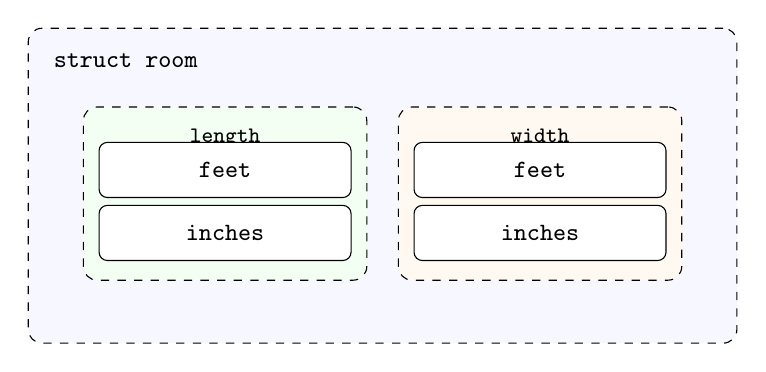
\begin{tikzpicture}[
    box/.style={draw, rounded corners=3pt, minimum width=3.2cm,
                minimum height=0.7cm, font=\small\ttfamily},
    outer/.style={draw, rounded corners=5pt, dashed, inner sep=10pt,
                  fill=blue!3},
    arr/.style={->, >=stealth, thick}
]
  % Room box
  \node[outer, minimum width=9cm, minimum height=4cm] (roombox) at (0,0) {};
  \node[font=\bfseries\small, anchor=north west] at (-4.3,1.8)
       {\texttt{struct room}};

  % Length
  \node[outer, minimum width=3.6cm, minimum height=2.2cm, fill=green!5]
       (lenbox) at (-2, -0.1) {};
  \node[font=\footnotesize\bfseries, anchor=north] at (-2, 0.85)
       {\texttt{length}};
  \node[box, fill=white] at (-2, 0.2) {feet};
  \node[box, fill=white] at (-2,-0.6) {inches};

  % Width
  \node[outer, minimum width=3.6cm, minimum height=2.2cm, fill=orange!5]
       (widbox) at (2, -0.1) {};
  \node[font=\footnotesize\bfseries, anchor=north] at (2, 0.85)
       {\texttt{width}};
  \node[box, fill=white] at (2, 0.2) {feet};
  \node[box, fill=white] at (2,-0.6) {inches};
\end{tikzpicture}
\end{center}

%-----------------------------------------------------------------------------
\section{Array of Structures}
\label{sec:struct-array}
%-----------------------------------------------------------------------------

\begin{definitionbox}{Array of Structures}
Since a \texttt{struct} defines a new data type, you can create an
\textbf{array of structures} just as you would create an array of
\texttt{int} or \texttt{float}.  Each element of the array is a
complete structure with all its members.
\end{definitionbox}

\noindent
The conceptual layout of an array of structures is shown below:

\begin{center}
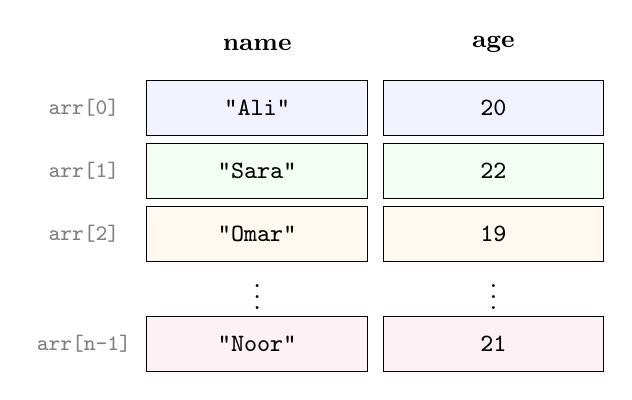
\begin{tikzpicture}[
    cell/.style={draw, minimum width=2.8cm, minimum height=0.7cm,
                 font=\small\ttfamily},
    idx/.style={font=\footnotesize\ttfamily, text=gray}
]
  % Column headers
  \node[font=\small\bfseries] at (0, 1.2)  {name};
  \node[font=\small\bfseries] at (3, 1.2)  {age};

  % Row 0
  \node[cell, fill=blue!5]   at (0, 0.4) {"Ali"};
  \node[cell, fill=blue!5]   at (3, 0.4) {20};
  \node[idx] at (-2.2, 0.4)  {arr[0]};

  % Row 1
  \node[cell, fill=green!5]  at (0, -0.4) {"Sara"};
  \node[cell, fill=green!5]  at (3, -0.4) {22};
  \node[idx] at (-2.2,-0.4)  {arr[1]};

  % Row 2
  \node[cell, fill=orange!5] at (0, -1.2) {"Omar"};
  \node[cell, fill=orange!5] at (3, -1.2) {19};
  \node[idx] at (-2.2,-1.2)  {arr[2]};

  % dots
  \node at (0, -1.9) {$\vdots$};
  \node at (3, -1.9) {$\vdots$};

  % Row n-1
  \node[cell, fill=purple!5] at (0, -2.6) {"Noor"};
  \node[cell, fill=purple!5] at (3, -2.6) {21};
  \node[idx] at (-2.2,-2.6)  {arr[n-1]};
\end{tikzpicture}
\end{center}

\subsection{Example 4 --- Array of Student Structures}

\begin{cppcode}
#include <iostream>
#include <cstring>
using namespace std;

struct student {
    char name[30];
    int  age;
};

int main() {
    const int SIZE = 3;
    student arr[SIZE];

    // Input
    for (int i = 0; i < SIZE; i++) {
        cout << "Enter name of student " << i + 1 << ": ";
        cin.getline(arr[i].name, 30);
        cout << "Enter age of student " << i + 1 << ":  ";
        cin  >> arr[i].age;
        cin.ignore(80, '\n');   // flush newline
    }

    // Output
    cout << "\n--- Student List ---" << endl;
    for (int i = 0; i < SIZE; i++) {
        cout << "Student " << i + 1 << ": "
             << arr[i].name << ", Age: "
             << arr[i].age  << endl;
    }

    return 0;
}
\end{cppcode}

\noindent
\textbf{Sample run:}
\begin{verbatim}
Enter name of student 1: Ali Hassan
Enter age of student 1:  20
Enter name of student 2: Sara Karim
Enter age of student 2:  22
Enter name of student 3: Omar Faris
Enter age of student 3:  19

--- Student List ---
Student 1: Ali Hassan, Age: 20
Student 2: Sara Karim, Age: 22
Student 3: Omar Faris, Age: 19
\end{verbatim}

\begin{infobox}{Accessing Members of Array Elements}
Use the array subscript followed by the dot operator:

\medskip
\texttt{arr[i].name} \qquad \texttt{arr[i].age}
\medskip

This first selects element \texttt{i} from the array and then
accesses the desired member of that element's structure.
\end{infobox}

\begin{conceptbox}{Structures vs.\ Arrays}
\renewcommand{\arraystretch}{1.3}
\begin{tabular}{@{} p{6.5cm} p{6.5cm} @{}}
\toprule
\textbf{Array} & \textbf{Structure} \\
\midrule
All elements must be of the \emph{same} data type.
    & Members can be of \emph{different} data types. \\
Elements are accessed by \textbf{index} (e.g.\ \texttt{a[0]}).
    & Members are accessed by \textbf{name} (e.g.\ \texttt{s.age}). \\
Useful for storing a collection of \emph{similar} items (e.g.\ 100
    marks). & Useful for grouping \emph{related but different}
    attributes (e.g.\ name, age, GPA). \\
Cannot be assigned directly with \texttt{=} in C-style arrays.
    & Can be assigned directly: \texttt{s2 = s1;} copies all members. \\
Fixed-size, determined at compile time.
    & Each variable holds one complete set of members. \\
\bottomrule
\end{tabular}
\end{conceptbox}
    % Structures

% ============================================================
%  WORKSHEETS (APPENDIX)
% ============================================================
\appendix
%=============================================================================
% Work Sheets (Appendix)
%=============================================================================
\chapter{Work Sheets}
\label{ch:worksheets}

%=============================================================================
\section{Work Sheet 5 --- Functions}
\label{ws:functions}
%=============================================================================

\begin{importantbox}{Instructions}
For each question below, write a complete C++ program.  Where a
\emph{function} is requested, implement the logic inside a
user-defined function and call it from \texttt{main()}.
\end{importantbox}

\begin{enumerate}[leftmargin=*, label=\textbf{Q\arabic*.}]

\item Write a program that reads 20 characters and uses a function to
      count and return how many of them are \textbf{uppercase} letters.

\item Write a function that receives a distance expressed in
      \textbf{feet and inches} and converts it to \textbf{meters}.\\
      \textit{Hint:} 1 foot = 12 inches, 1 inch = 2.54\,cm.

\item Write a function that receives a total number of \textbf{seconds}
      and converts it to the format \texttt{hr:mn:sec}.  For example,
      3661 seconds $\rightarrow$ \texttt{1:1:1}.

\item Write a function that takes an integer and determines whether it
      is \textbf{odd} or \textbf{even}.

\item Write a function that computes the \textbf{permutation}
      $P(n) = n!$ of a given positive integer~$n$.

\item Write a function that receives a student's mark and returns the
      corresponding \textbf{grade point} according to the following
      scale:

      \begin{center}
      \renewcommand{\arraystretch}{1.2}
      \begin{tabular}{@{} c c @{}}
      \toprule
      \textbf{Mark Range} & \textbf{Grade Point} \\
      \midrule
      90--100 & 4 \\
      80--89  & 3 \\
      70--79  & 2 \\
      60--69  & 1 \\
      Below 60 & 0 \\
      \bottomrule
      \end{tabular}
      \end{center}

\item Write a program that uses a function to compute and print the
      first $n$ terms of the \textbf{Fibonacci} sequence:\\
      $0,\ 1,\ 1,\ 2,\ 3,\ 5,\ 8,\ 13,\ \ldots$

\item Write a function that receives an integer $n$ and returns its
      \textbf{factorial} ($n!$).

\item Using a factorial function, evaluate
      \[
          z = \frac{x! - y!}{(x - y)!}
      \]
      for user-supplied values of $x$ and $y$ (where $x \geq y$).

\item Write a function that receives a \textbf{year} and determines
      whether it is a \textbf{leap year}.\\
      \textit{Rule:} A year is a leap year if it is divisible by~4,
      except for century years which must also be divisible by~400.

\item Write a program that reads two integers $x$ and $y$ and uses the
      library function \texttt{pow()} to compute $x^{y}$.

\item Write a function that receives an integer and returns its
      \textbf{reverse}.  For example, $765432 \rightarrow 234567$.

\item Write a program that uses functions to read the marks of
      \textbf{8~students}, then compute and display their \textbf{sum}
      and \textbf{average}.

\item Write a function that receives a character and \textbf{converts
      its case} --- uppercase to lowercase or vice versa --- and returns
      the result.

\item Write a \textbf{recursive} function that computes $n^{p}$
      (the power of $n$ raised to $p$) without using
      \texttt{pow()}.\\
      \textit{Hint:} $n^{p} = n \times n^{p-1}$, with base case
      $n^{0} = 1$.

\end{enumerate}

\newpage
%=============================================================================
\section{Work Sheet 6 --- Arrays}
\label{ws:arrays}
%=============================================================================

\begin{importantbox}{Instructions}
For each question below, write a complete C++ program.  Use arrays as
specified; you may use functions where appropriate.
\end{importantbox}

\begin{enumerate}[leftmargin=*, label=\textbf{Q\arabic*.}]

\item Write a program that reads an array of $n$ integers and checks
      whether the array is \textbf{sorted in ascending order}.

\item Write a program that reads an array of $n$ integers and counts
      the number of elements that are equal to \textbf{zero}.

\item Write a program that reads two integer arrays of the same size
      and produces a third array that is their element-wise
      \textbf{sum}.

\item Write a program that reads an integer array and creates a new
      array in which every element is \textbf{multiplied by~2}.

\item Write a program that reads the daily temperatures for one week
      (7 values) into an array, then computes and prints the
      \textbf{average temperature}.

\item Write a program that reads two sorted arrays and \textbf{merges}
      them into a single sorted array.

\item Write a program that reads a $3 \times 4$ matrix and computes
      the \textbf{sum of each column}.

\item Write a program that reads a square matrix of order $n$ and
      computes the \textbf{sum of the main diagonal} elements.

\item Write a program that reads a square matrix of order $n$ and
      computes the \textbf{sum of the secondary diagonal} elements.

\item Write a program that reads a $4 \times 5$ matrix and
      \textbf{searches} for a user-supplied value, reporting its
      position (row and column) if found.

\item Write a program that reads a one-dimensional array of 12 elements
      and stores them into a $3 \times 4$ two-dimensional array
      (\textbf{1-D to 2-D conversion}).

\item Write a program that reads a character array and \textbf{splits}
      it into two arrays: one containing the letters and the other
      containing the digits.

\item Write a program that reads an integer array and replaces every
      element that is both \textbf{even} and \textbf{positive} with
      the value~\textbf{10}.  Print the array before and after the
      replacement.

\item Write a program that reads a square matrix and replaces every
      \textbf{even} element on the \textbf{main diagonal} with~0.
      Print the matrix before and after.

\item Write a program that reads a $4 \times 5$ matrix and finds the
      \textbf{minimum element} in the entire matrix, printing its value
      and position (row and column).

\item Write a program that reads a $3 \times 3$ matrix and
      \textbf{exchanges} (swaps) two user-specified \textbf{rows}.
      Print the matrix before and after the swap.

\item Write a program that reads a $3 \times 3$ matrix and
      \textbf{exchanges} (swaps) a user-specified \textbf{row} with a
      user-specified \textbf{column}.  Print the matrix before and
      after.

\item Write a program that reads an array of $n$ integers and performs
      a \textbf{left rotation} by one position.  For example,
      $\{1,2,3,4,5\} \rightarrow \{2,3,4,5,1\}$.

\item Write a program that reads an array of $n$ integers and
      \textbf{deletes} the element at a user-specified position,
      shifting subsequent elements to fill the gap.

\item Write a program that reads an array of $n$ integers and sorts it
      in \textbf{ascending} order.

\item Write a program that reads an array of $n$ integers and sorts it
      in \textbf{descending} order.

\item Write a program that reads an array of $n$ integers and computes
      the \textbf{average of the even} numbers only.

\item Write a program that reads a $3 \times 4$ matrix~$A$ and creates
      a one-dimensional array~$B$ of size~3 such that each element
      $B[i]$ is the \textbf{sum of row~$i$} of~$A$.

      \textit{Example:}
\begin{verbatim}
A = | 1  2  3  4 |    B = | 10 |
    | 5  6  7  8 |        | 26 |
    | 9 10 11 12 |        | 42 |
\end{verbatim}

\item Write a program that reads a square matrix of order $n$ and
      finds the \textbf{greatest element on the secondary diagonal}.

\item Write a program that creates and prints each of the following
      arrays (the user supplies the size~$n$):

      \begin{enumerate}[label=(\alph*)]
        \item An array containing the first $n$ \textbf{even} numbers:
              $\{2, 4, 6, 8, \ldots\}$
        \item An array containing the first $n$ \textbf{odd} numbers:
              $\{1, 3, 5, 7, \ldots\}$
        \item An array whose elements follow the pattern
              $\{1, 2, 4, 8, 16, \ldots\}$ (powers of~2).
      \end{enumerate}

\end{enumerate}

\newpage
%=============================================================================
\section{Work Sheet 7 --- Strings}
\label{ws:strings}
%=============================================================================

\begin{importantbox}{Instructions}
For each question below, write a complete C++ program using C-style
strings (\texttt{char} arrays).  Make use of the string I/O and
library functions discussed in Chapter~\ref{ch:strings}.
\end{importantbox}

\begin{enumerate}[leftmargin=*, label=\textbf{Q\arabic*.}]

\item Write a program that reads a string from the user, prints the
      complete string, and then prints its characters in
      \textbf{reverse order} (one character per line).

      \textit{Example:}
\begin{verbatim}
Input:  Hello
Output: Hello
        o
        l
        l
        e
        H
\end{verbatim}

\item Write a program that reads a string and \textbf{swaps the case}
      of every letter --- uppercase letters become lowercase and vice
      versa.  Non-letter characters remain unchanged.

      \textit{Example:}
\begin{verbatim}
Input:  Hello World 123
Output: hELLO wORLD 123
\end{verbatim}

\item Write a program that reads a full sentence (using
      \texttt{cin.getline()}) and prints each \textbf{word on a
      separate line}.  Assume words are separated by single spaces.

      \textit{Example:}
\begin{verbatim}
Input:  Structured Programming in C++
Output: Structured
        Programming
        in
        C++
\end{verbatim}

\item Write a program that demonstrates the use of the following
      \textbf{I/O functions}:
      \begin{itemize}
        \item \texttt{cin.getline()} --- to read a full line,
        \item \texttt{cin.get()} --- to read a single character,
        \item \texttt{cin.ignore()} --- to discard remaining input,
        \item \texttt{cin.putback()} --- to push a character back,
        \item \texttt{cout.put()} --- to output a single character.
      \end{itemize}
      Display appropriate messages so the output clearly shows which
      function is being used.

\item Write a program that demonstrates the use of the following
      \textbf{string library functions}:
      \begin{itemize}
        \item \texttt{strlen()} --- to find the length of a string,
        \item \texttt{strcpy()} --- to copy one string into another,
        \item \texttt{strcat()} --- to concatenate two strings,
        \item \texttt{strcmp()} --- to compare two strings.
      \end{itemize}
      Read two strings from the user and apply each function, printing
      the result after every operation.

\end{enumerate}


\end{document}
